% Options for packages loaded elsewhere
\PassOptionsToPackage{unicode}{hyperref}
\PassOptionsToPackage{hyphens}{url}
%
\documentclass[
]{book}
\usepackage{amsmath,amssymb}
\usepackage{iftex}
\ifPDFTeX
  \usepackage[T1]{fontenc}
  \usepackage[utf8]{inputenc}
  \usepackage{textcomp} % provide euro and other symbols
\else % if luatex or xetex
  \usepackage{unicode-math} % this also loads fontspec
  \defaultfontfeatures{Scale=MatchLowercase}
  \defaultfontfeatures[\rmfamily]{Ligatures=TeX,Scale=1}
\fi
\usepackage{lmodern}
\ifPDFTeX\else
  % xetex/luatex font selection
\fi
% Use upquote if available, for straight quotes in verbatim environments
\IfFileExists{upquote.sty}{\usepackage{upquote}}{}
\IfFileExists{microtype.sty}{% use microtype if available
  \usepackage[]{microtype}
  \UseMicrotypeSet[protrusion]{basicmath} % disable protrusion for tt fonts
}{}
\makeatletter
\@ifundefined{KOMAClassName}{% if non-KOMA class
  \IfFileExists{parskip.sty}{%
    \usepackage{parskip}
  }{% else
    \setlength{\parindent}{0pt}
    \setlength{\parskip}{6pt plus 2pt minus 1pt}}
}{% if KOMA class
  \KOMAoptions{parskip=half}}
\makeatother
\usepackage{xcolor}
\usepackage{color}
\usepackage{fancyvrb}
\newcommand{\VerbBar}{|}
\newcommand{\VERB}{\Verb[commandchars=\\\{\}]}
\DefineVerbatimEnvironment{Highlighting}{Verbatim}{commandchars=\\\{\}}
% Add ',fontsize=\small' for more characters per line
\usepackage{framed}
\definecolor{shadecolor}{RGB}{248,248,248}
\newenvironment{Shaded}{\begin{snugshade}}{\end{snugshade}}
\newcommand{\AlertTok}[1]{\textcolor[rgb]{0.94,0.16,0.16}{#1}}
\newcommand{\AnnotationTok}[1]{\textcolor[rgb]{0.56,0.35,0.01}{\textbf{\textit{#1}}}}
\newcommand{\AttributeTok}[1]{\textcolor[rgb]{0.13,0.29,0.53}{#1}}
\newcommand{\BaseNTok}[1]{\textcolor[rgb]{0.00,0.00,0.81}{#1}}
\newcommand{\BuiltInTok}[1]{#1}
\newcommand{\CharTok}[1]{\textcolor[rgb]{0.31,0.60,0.02}{#1}}
\newcommand{\CommentTok}[1]{\textcolor[rgb]{0.56,0.35,0.01}{\textit{#1}}}
\newcommand{\CommentVarTok}[1]{\textcolor[rgb]{0.56,0.35,0.01}{\textbf{\textit{#1}}}}
\newcommand{\ConstantTok}[1]{\textcolor[rgb]{0.56,0.35,0.01}{#1}}
\newcommand{\ControlFlowTok}[1]{\textcolor[rgb]{0.13,0.29,0.53}{\textbf{#1}}}
\newcommand{\DataTypeTok}[1]{\textcolor[rgb]{0.13,0.29,0.53}{#1}}
\newcommand{\DecValTok}[1]{\textcolor[rgb]{0.00,0.00,0.81}{#1}}
\newcommand{\DocumentationTok}[1]{\textcolor[rgb]{0.56,0.35,0.01}{\textbf{\textit{#1}}}}
\newcommand{\ErrorTok}[1]{\textcolor[rgb]{0.64,0.00,0.00}{\textbf{#1}}}
\newcommand{\ExtensionTok}[1]{#1}
\newcommand{\FloatTok}[1]{\textcolor[rgb]{0.00,0.00,0.81}{#1}}
\newcommand{\FunctionTok}[1]{\textcolor[rgb]{0.13,0.29,0.53}{\textbf{#1}}}
\newcommand{\ImportTok}[1]{#1}
\newcommand{\InformationTok}[1]{\textcolor[rgb]{0.56,0.35,0.01}{\textbf{\textit{#1}}}}
\newcommand{\KeywordTok}[1]{\textcolor[rgb]{0.13,0.29,0.53}{\textbf{#1}}}
\newcommand{\NormalTok}[1]{#1}
\newcommand{\OperatorTok}[1]{\textcolor[rgb]{0.81,0.36,0.00}{\textbf{#1}}}
\newcommand{\OtherTok}[1]{\textcolor[rgb]{0.56,0.35,0.01}{#1}}
\newcommand{\PreprocessorTok}[1]{\textcolor[rgb]{0.56,0.35,0.01}{\textit{#1}}}
\newcommand{\RegionMarkerTok}[1]{#1}
\newcommand{\SpecialCharTok}[1]{\textcolor[rgb]{0.81,0.36,0.00}{\textbf{#1}}}
\newcommand{\SpecialStringTok}[1]{\textcolor[rgb]{0.31,0.60,0.02}{#1}}
\newcommand{\StringTok}[1]{\textcolor[rgb]{0.31,0.60,0.02}{#1}}
\newcommand{\VariableTok}[1]{\textcolor[rgb]{0.00,0.00,0.00}{#1}}
\newcommand{\VerbatimStringTok}[1]{\textcolor[rgb]{0.31,0.60,0.02}{#1}}
\newcommand{\WarningTok}[1]{\textcolor[rgb]{0.56,0.35,0.01}{\textbf{\textit{#1}}}}
\usepackage{longtable,booktabs,array}
\usepackage{calc} % for calculating minipage widths
% Correct order of tables after \paragraph or \subparagraph
\usepackage{etoolbox}
\makeatletter
\patchcmd\longtable{\par}{\if@noskipsec\mbox{}\fi\par}{}{}
\makeatother
% Allow footnotes in longtable head/foot
\IfFileExists{footnotehyper.sty}{\usepackage{footnotehyper}}{\usepackage{footnote}}
\makesavenoteenv{longtable}
\usepackage{graphicx}
\makeatletter
\newsavebox\pandoc@box
\newcommand*\pandocbounded[1]{% scales image to fit in text height/width
  \sbox\pandoc@box{#1}%
  \Gscale@div\@tempa{\textheight}{\dimexpr\ht\pandoc@box+\dp\pandoc@box\relax}%
  \Gscale@div\@tempb{\linewidth}{\wd\pandoc@box}%
  \ifdim\@tempb\p@<\@tempa\p@\let\@tempa\@tempb\fi% select the smaller of both
  \ifdim\@tempa\p@<\p@\scalebox{\@tempa}{\usebox\pandoc@box}%
  \else\usebox{\pandoc@box}%
  \fi%
}
% Set default figure placement to htbp
\def\fps@figure{htbp}
\makeatother
\setlength{\emergencystretch}{3em} % prevent overfull lines
\providecommand{\tightlist}{%
  \setlength{\itemsep}{0pt}\setlength{\parskip}{0pt}}
\setcounter{secnumdepth}{5}
\usepackage{booktabs}
\usepackage[]{natbib}
\bibliographystyle{apalike}
\usepackage{bookmark}
\IfFileExists{xurl.sty}{\usepackage{xurl}}{} % add URL line breaks if available
\urlstyle{same}
\hypersetup{
  pdftitle={First Steps in R},
  pdfauthor={MASH},
  hidelinks,
  pdfcreator={LaTeX via pandoc}}

\title{First Steps in R}
\author{MASH}
\date{2026-09-16}

\begin{document}
\maketitle

{
\setcounter{tocdepth}{1}
\tableofcontents
}
\chapter{About}\label{about}

What this book is about

\chapter{Everything you need to know before you learn R}\label{everything-you-need-to-know-before-you-learn-r}

If you are completely new to R, you are in the right place.

Learning R can feel intimidating at first. Unlike software such as Excel and SPSS, R asks you to \textbf{type instructions} to tell the computer what you want it to do rather than clicking icons and menus.

That can feel strange at first.

The good news is that you do \textbf{not} need to be a programmer to learn R. You just need to learn a few basic ideas, practise them, and gradually build up your understanding.

This document is not intended to teach you R - rather, it should help you get started and highlight the key concepts to know before you try to learn R.

By the end, you should understand:

\begin{itemize}
\tightlist
\item
  What R is
\item
  The difference between R and Rstudio
\item
  Some advantages and disadvantages of R versus other software
\item
  Main parts of the RStudio interface
\item
  How to begin coding in R
\item
  Where to find help and learning materials
\item
  How to continue learning R independently
\end{itemize}

\begin{quote}
\textbf{The most important thing to remember:} You do not need to understand everything before you start. Learning R is a process.
\end{quote}

\section{What is R?}\label{what-is-r}

R is a \textbf{programming language}. That means that instead of telling R what to do by clicking buttons in a menu, you generally type instructions.

For example, you can ask R to calculate 2+2

\begin{Shaded}
\begin{Highlighting}[]
\DecValTok{2} \SpecialCharTok{+} \DecValTok{2}
\end{Highlighting}
\end{Shaded}

and it will return:

\begin{verbatim}
#> [1] 4
\end{verbatim}

R is widely used for statistics, data analysis and data visualisation. It is used by students, researchers, universities, governments, businesses and many other organisations.

R is especially useful when you need to:

\begin{itemize}
\tightlist
\item
  Work with data
\item
  Perform calculations
\item
  Carry out statistical analyses
\item
  Create graphs and visualisations
\item
  Manipulate datasets
\end{itemize}

\subsection{What is RStudio?}\label{what-is-rstudio}

You will often hear people talk about \textbf{R and RStudio} as though they are the same thing.

They are not.

\textbf{R is the programming language itself.} It is the thing that actually performs your calculations, analyses and commands.

\textbf{RStudio is an Integrated Development Environment (IDE) for R.} A fancy term for a user dashboard. It provides a convenient interface for working with R.

💡 \textbf{Think of it this way:}
If R is the engine, RStudio is the dashboard that makes the engine easier to use.

You can use R without RStudio, but RStudio provides a much more convenient environment for writing, running and organising R code.

When you are getting started, you will normally install \textbf{both R and RStudio}.

\subsection{Why learn R?}\label{why-learn-r}

There are lots of reasons to learn R.

\subsubsection{It's free!}\label{its-free}

One of the biggest advantages of R is that it is \textbf{free}. You do not need to buy a licence to continue using R after you graduate and there are no limits to how many devices you install it on.

\subsubsection{It's flexible!}\label{its-flexible}

R can be used for an enormous range of tasks from calculating statistics, plotting data, statistical analysis, hypothesis tests, regression, automating tasks, writing reports and much more.

\subsubsection{It's widely used!}\label{its-widely-used}

R is widely used in scientific research and academia, as well as industry. R has an enormous library of \textbf{packages} to help you perform even quite specific tasks.

Packages are collections of additional functions, data and other resources that extend what R can do.

\begin{quote}
\textbf{R can do a huge amount. And if it cannot already do something you need, there is often a package that can help --- or you can potentially create your own solution.}
\end{quote}

\subsection{The downsides of R}\label{the-downsides-of-r}

R is powerful, but there are some things that can make it difficult to use when you first start. The main thing being that you have to interact with it as a programming language.

If you are used to software where you select options from menus, R may initially feel unfamiliar and there will initially be quite a lot to learn.

Before being proficient in R, you will need to learn:

\begin{itemize}
\tightlist
\item
  How R understands commands
\item
  What objects are
\item
  How functions work
\item
  How to structure your code
\item
  How to find and fix errors
\end{itemize}

This can feel daunting at first but is ** completely normal.**

The first few sessions of learning R are often the hardest because you are learning a new way of communicating with a computer.

In software such as Excel, to plot a graph you might:

\begin{enumerate}
\def\labelenumi{\arabic{enumi}.}
\tightlist
\item
  select some cells;
\item
  click \emph{insert};
\item
  select the chart type you want;
\item
  click OK.
\end{enumerate}

In R, you might instead type something like:

\begin{Shaded}
\begin{Highlighting}[]
\FunctionTok{boxplot}\NormalTok{(my\_data)}
\end{Highlighting}
\end{Shaded}

and get a plot such as

\pandocbounded{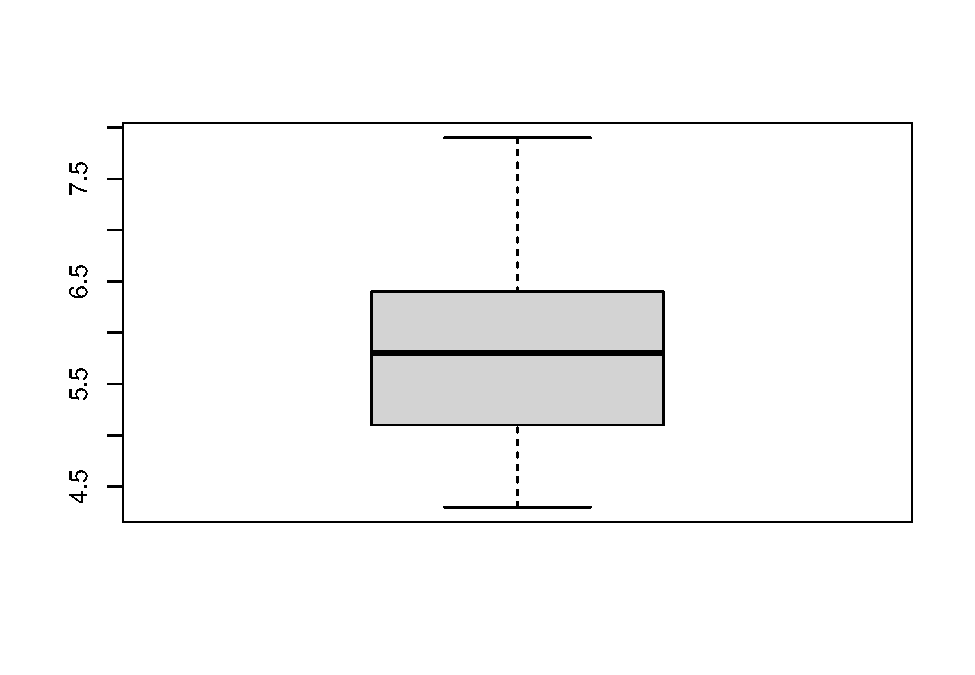
\includegraphics[keepaspectratio]{01_EYNTKBYLR_files/figure-latex/unnamed-chunk-5-1.pdf}}

\section{Installing R and RStudio}\label{installing-r-and-rstudio}

The \href{https://sheffield.ac.uk/mash/stats-resources/r}{University of Sheffield MASH R resources page} contains a guide to downloading and setting up both \href{https://cran.r-project.org/}{R} and \href{https://posit.co/products/open-source/rstudio}{RStudio}.

Alternatively, go to both the \href{https://cran.r-project.org/}{R} and \href{https://posit.co/products/open-source/rstudio}{RStudio} webpages and download the appropriate version for your device.

\section{Getting to know RStudio}\label{getting-to-know-rstudio}

When you open RStudio, you will probably see several different sections or \textbf{panes}.

The exact arrangement can vary depending on your version and settings.

A common layout contains four main panes:

\begin{enumerate}
\def\labelenumi{\arabic{enumi}.}
\tightlist
\item
  (Top-left) \textbf{Source}
\item
  (Bottom-left) \textbf{Console}
\item
  (Top-right) \textbf{Environment / History}
\item
  (Bottom-left) \textbf{Files / Plots / Packages / Help}
\end{enumerate}

\subsection{1. Source}\label{source}

The \textbf{Source} pane is where you can write, edit and save your code. If it is the first time opening Rstudio, the \textbf{Source} pane may not appear until you click the following.

File \textgreater{} New File \textgreater{} R Script

The \textbf{Source pane} is where you should normally develop your analysis. The saved code is referred to as a script and has the file extension \texttt{.R}. These files can be reopened and worked on at any time.

\subsection{2. Console}\label{console}

The \textbf{Console} is where R receives and executes commands.

You can type directly into it. The result will appear underneath. Unlike an R script, the \textbf{Console} is temporary and anything you type into it is not saved. The \textbf{Console} is particularly useful for:

\begin{itemize}
\tightlist
\item
  Trying out commands
\item
  Testing ideas
\item
  Checking the result of a function
\item
  Troubleshooting
\end{itemize}

\begin{quote}
Tip: you can press the \textbf{Up} key with your cursor in the Console to quickly cycle through commands you have typed recently**
\end{quote}

\subsection{3. Environment / History}\label{environment-history}

The \textbf{Environment} pane shows objects that currently exist in your R session.

For example, if you run the code:

\begin{Shaded}
\begin{Highlighting}[]
\NormalTok{student\_scores }\OtherTok{\textless{}{-}} \FunctionTok{c}\NormalTok{(}\DecValTok{65}\NormalTok{, }\DecValTok{72}\NormalTok{, }\DecValTok{81}\NormalTok{, }\DecValTok{69}\NormalTok{, }\DecValTok{88}\NormalTok{)}
\end{Highlighting}
\end{Shaded}

the object \texttt{student\_scores} will appear in the \textbf{Environment}. \emph{We'll talk more about objects later}.

The \textbf{Environment} therefore gives you a useful overview of the objects you have created.

There are other tabs within this pane, the next most useful being the \textbf{History} tab which shows all the commands that you have previously entered.

This can be useful when you are trying to remember something you did earlier in your session.

\subsection{4. Files / Plots / Packages / Help}\label{files-plots-packages-help}

The last window contains several tabs including \textbf{Files, Plots, Packages and Help}.

The \textbf{Files} tab allows you to navigate through folders on your computer (see \textbf{Working Directories} for more detail).

\textbf{Plots} displays graphs that you create in R.

\textbf{Packages} allows you to see packages that are installed in your R session.

\textbf{Help} displays R's documentation when you request it using the \texttt{?} command (see \hyperref[Errors]{Errors} for further help).

The following table summarises the pane functions.

\begin{longtable}[]{@{}ll@{}}
\toprule\noalign{}
Window & What it does \\
\midrule\noalign{}
\endhead
\bottomrule\noalign{}
\endlastfoot
\textbf{Source} & Write and edit R scripts \\
\textbf{Console} & Run R commands \\
\textbf{Environment} & View objects currently stored in R \\
\textbf{History} & View previously entered commands \\
\textbf{Files} & Navigate through files and folders \\
\textbf{Plots} & View graphs \\
\textbf{Packages} & Install and manage packages \\
\textbf{Help} & Access R documentation \\
\end{longtable}

\subsection{Working directories}\label{working-directories}

One concept that often causes confusion when you first start using R is the \textbf{working directory}.

The \textbf{working directory} is the folder that R is currently using as its default location for reading and writing files.

You can find your current working directory by running:

\begin{Shaded}
\begin{Highlighting}[]
\FunctionTok{getwd}\NormalTok{()}
\end{Highlighting}
\end{Shaded}

\texttt{getwd()} means \textbf{get working directory}.

You can change the working directory using \texttt{setwd()} and the path to your desired folder. For example:

\begin{Shaded}
\begin{Highlighting}[]
\FunctionTok{setwd}\NormalTok{(}\StringTok{"C:/Users/YourName/Documents/R"}\NormalTok{)}
\end{Highlighting}
\end{Shaded}

The exact path will depend on your computer.

\begin{quote}
\textbf{Tip:} You do not necessarily need to use \texttt{setwd()}. Instead, in the \textbf{Files} tab, click \textbf{\ldots{}} on the right-hand side, click through the file explorer to find the folder you want then click \textbf{Open}. Click the cog symbol titled \textbf{More} then Select \textbf{Set as Working Directory}.
\end{quote}

\section{Learning how to write code}\label{learning-how-to-write-code}

There are a few things that are worth understanding right at the beginning.

R is primarily controlled by typing commands. You can think of each line of R code as an instruction.

For example, to find the mean of the \texttt{student\_scores} given above you'd type:

\begin{Shaded}
\begin{Highlighting}[]
\FunctionTok{mean}\NormalTok{(student\_scores)}
\end{Highlighting}
\end{Shaded}

It is very important before learning R to realise that \textbf{you do not have to memorise everything.}

One of the most important skills in R is knowing how to find information. It is unlikely that you will remember the code for everything you want to do.

That is normal.

Learning R is not about memorising an enormous list of commands. It is about learning enough of the language that you can understand, debug (fix) and build code.

The \href{https://sheffield.ac.uk/mash/stats-resources/r\#First-steps}{University of Sheffield MASH R resources page} provides first steps in R.

These first steps will guide you through:

\begin{itemize}
\tightlist
\item
  Installing R
\item
  Downloading RStudio
\item
  Interacting with R
\item
  Understanding objects and functions
\item
  Working with vectors
\item
  Getting started with data
\item
  Installing packages
\end{itemize}

These are a good place to get started!

\subsection{What is a command?}\label{what-is-a-command}

A \textbf{command} is an instruction that you give to R.

To run a command in the \textbf{Console} you simply type your command and press \textbf{Enter}.

To run a command in the \textbf{Source} pane (script) there are two ways:

\begin{itemize}
\item
  Highlight the line(s) of code and press \textbf{Ctrl + Enter} on your keyboard or the \textbf{Run} key in the top right of the Source pane.
\item
  Put your cursor on the line of code and press \textbf{Ctrl + Enter}. This also moves the cursor to the next line so you can easily run the next line.
\end{itemize}

\begin{quote}
Tip: To quickly highlight your entire script click \textbf{Ctrl + A} with your cursor anywhere in the script.
\end{quote}

An example command is:

\begin{Shaded}
\begin{Highlighting}[]
\DecValTok{2} \SpecialCharTok{+} \DecValTok{2}
\end{Highlighting}
\end{Shaded}

an instruction asking R to add two numbers.

Another example is:

\begin{Shaded}
\begin{Highlighting}[]
\NormalTok{even\_numbers }\OtherTok{\textless{}{-}} \FunctionTok{c}\NormalTok{(}\DecValTok{2}\NormalTok{, }\DecValTok{4}\NormalTok{, }\DecValTok{6}\NormalTok{, }\DecValTok{8}\NormalTok{)}
\end{Highlighting}
\end{Shaded}

This tells R to create an \emph{object} named \texttt{even\_numbers} by combing the numbers 2,4,6 and 8. Note here, that in programming we call this a vector. Vectors are formed in R using the function \texttt{c()} where \texttt{c} stands for combine.

You will quickly become familiar with the basic structure of R commands.

\subsection{What is a function?}\label{what-is-a-function}

A \textbf{function} is a piece of code designed to perform a particular task.

Functions are one of the most important concepts in R.

For example:

\begin{Shaded}
\begin{Highlighting}[]
\FunctionTok{mean}\NormalTok{(}\FunctionTok{c}\NormalTok{(}\DecValTok{2}\NormalTok{, }\DecValTok{4}\NormalTok{, }\DecValTok{6}\NormalTok{, }\DecValTok{8}\NormalTok{))}
\end{Highlighting}
\end{Shaded}

gives the following output.

\begin{verbatim}
#> [1] 5
\end{verbatim}

Here:

\begin{itemize}
\tightlist
\item
  \texttt{mean} is the function;
\item
  \texttt{c(2,\ 4,\ 6,\ 8)} is the input;
\item
  the function calculates the mean.
\end{itemize}

Functions are generally followed by parentheses:

\begin{Shaded}
\begin{Highlighting}[]
\FunctionTok{function\_name}\NormalTok{()}
\end{Highlighting}
\end{Shaded}

The information that you give to a function is called an \textbf{argument}.

For example:

\begin{Shaded}
\begin{Highlighting}[]
\FunctionTok{round}\NormalTok{(}\FloatTok{3.14159}\NormalTok{, }\AttributeTok{digits =} \DecValTok{2}\NormalTok{)}
\CommentTok{\#\textgreater{} [1] 3.14}
\end{Highlighting}
\end{Shaded}

Here:

\begin{itemize}
\tightlist
\item
  \texttt{round()} is the function;
\item
  \texttt{3.14159} is the value being rounded;
\item
  \texttt{digits\ =\ 2} tells R how many decimal places to use.
\end{itemize}

\subsection{Objects}\label{objects}

Objects are another fundamental idea in R.

An object is something that R can store and work with.

For example:

\begin{Shaded}
\begin{Highlighting}[]
\NormalTok{age }\OtherTok{\textless{}{-}} \DecValTok{21}
\end{Highlighting}
\end{Shaded}

Here we have created an object called \texttt{age}.

We can then ask R to show us its value:

\begin{Shaded}
\begin{Highlighting}[]
\NormalTok{age}
\CommentTok{\#\textgreater{} [1] 21}
\end{Highlighting}
\end{Shaded}

We can also use it in another calculation:

\begin{Shaded}
\begin{Highlighting}[]
\NormalTok{age }\SpecialCharTok{+} \DecValTok{1}
\CommentTok{\#\textgreater{} [1] 22}
\end{Highlighting}
\end{Shaded}

\subsubsection{Assignment}\label{assignment}

The \texttt{\textless{}-} symbol is commonly used to assign a value to an object.

For example:

\begin{Shaded}
\begin{Highlighting}[]
\NormalTok{my\_number }\OtherTok{\textless{}{-}} \DecValTok{10}
\end{Highlighting}
\end{Shaded}

This means store the value \texttt{10} in an object called \texttt{my\_number}.

Objects can contain different types of information. They do not have to contain just single numbers.

For example, an object can contain text:

\begin{Shaded}
\begin{Highlighting}[]
\NormalTok{student\_name }\OtherTok{\textless{}{-}} \StringTok{"Alex"}
\end{Highlighting}
\end{Shaded}

Or several numbers:

\begin{Shaded}
\begin{Highlighting}[]
\NormalTok{test\_scores }\OtherTok{\textless{}{-}} \FunctionTok{c}\NormalTok{(}\DecValTok{65}\NormalTok{, }\DecValTok{72}\NormalTok{, }\DecValTok{81}\NormalTok{, }\DecValTok{69}\NormalTok{, }\DecValTok{88}\NormalTok{)}
\end{Highlighting}
\end{Shaded}

For now, the important thing is simply to understand that R allows you to \textbf{store information in objects and then use those objects later}.

\subsubsection{Naming objects}\label{naming-objects}

It is a good idea to give objects sensible names. When naming objects, best practices are to:

\begin{enumerate}
\def\labelenumi{\arabic{enumi}.}
\tightlist
\item
  Be informative about that the object represents
\item
  Do not use spaces
\item
  If it has multiple words in the name, separate these by underscores or capitalise each word.
\item
  Do not include dots or other symbols
\end{enumerate}

Good examples are:

\begin{Shaded}
\begin{Highlighting}[]
\NormalTok{age }\OtherTok{\textless{}{-}} \DecValTok{21}
\NormalTok{average\_score }\OtherTok{\textless{}{-}} \DecValTok{75}
\NormalTok{TestScores }\OtherTok{\textless{}{-}} \FunctionTok{c}\NormalTok{(}\DecValTok{65}\NormalTok{, }\DecValTok{72}\NormalTok{, }\DecValTok{81}\NormalTok{, }\DecValTok{69}\NormalTok{, }\DecValTok{88}\NormalTok{)}
\end{Highlighting}
\end{Shaded}

Compared with bad names:

\begin{Shaded}
\begin{Highlighting}[]
\NormalTok{x }\OtherTok{\textless{}{-}} \DecValTok{21}
\NormalTok{average score }\OtherTok{\textless{}{-}} \DecValTok{75}
\NormalTok{TEST.SCORES}\SpecialCharTok{!} \ErrorTok{\textless{}}\SpecialCharTok{{-}}  \FunctionTok{c}\NormalTok{(}\DecValTok{65}\NormalTok{, }\DecValTok{72}\NormalTok{, }\DecValTok{81}\NormalTok{, }\DecValTok{69}\NormalTok{, }\DecValTok{88}\NormalTok{)}
\end{Highlighting}
\end{Shaded}

The last two objects \texttt{average\ score} and \texttt{TEST.SCORES!} are so bad that they will give you the following error!

\begin{verbatim}
#> Error in parse(text = input): <text>:1:9: unexpected symbol
#> 1: average score
#>             ^
\end{verbatim}

\subsection{Comments}\label{comments}

You can add comments to your R code using the \texttt{\#} symbol.

Anything after \texttt{\#} on that line will be treated as a comment rather than R code and wont be executed when you run that line or script.

For example:

\begin{Shaded}
\begin{Highlighting}[]
\CommentTok{\# Calculate the mean of the scores}
\NormalTok{scores }\OtherTok{\textless{}{-}} \FunctionTok{c}\NormalTok{(}\DecValTok{1}\NormalTok{,}\DecValTok{2}\NormalTok{,}\DecValTok{3}\NormalTok{,}\DecValTok{4}\NormalTok{,}\DecValTok{5}\NormalTok{)}
\FunctionTok{mean}\NormalTok{(scores)}
\end{Highlighting}
\end{Shaded}

Comments are useful for explaining what your code is doing.

You can also use comments to organise a script:

\begin{Shaded}
\begin{Highlighting}[]
\CommentTok{\# {-}{-}{-}{-}{-}{-}{-}{-}{-}{-}{-}{-}{-}{-}{-}{-}{-}{-}{-}{-}{-}{-}{-}{-}{-}{-}{-}{-}{-}{-}{-}{-}{-}{-}{-}}
\CommentTok{\# Calculate summary statistics}
\CommentTok{\# {-}{-}{-}{-}{-}{-}{-}{-}{-}{-}{-}{-}{-}{-}{-}{-}{-}{-}{-}{-}{-}{-}{-}{-}{-}{-}{-}{-}{-}{-}{-}{-}{-}{-}{-}}
\FunctionTok{mean}\NormalTok{(scores)}
\FunctionTok{median}\NormalTok{(scores)}
\FunctionTok{sd}\NormalTok{(scores)}
\end{Highlighting}
\end{Shaded}

\begin{quote}
\textbf{Good habit:} Write comments that help you --- and someone else --- understand what your code is doing.
\end{quote}

Keeping your code organised. As your R scripts become longer, organisation becomes increasingly important.

You can use comments and headings to divide your code into sections.

For example:

\begin{Shaded}
\begin{Highlighting}[]
\CommentTok{\# Load packages}

\FunctionTok{library}\NormalTok{(ggplot2)}

\CommentTok{\# Import data}

\NormalTok{data }\OtherTok{\textless{}{-}} \FunctionTok{read.csv}\NormalTok{(}\StringTok{"my\_data.csv"}\NormalTok{)}

\CommentTok{\# Explore data}

\FunctionTok{head}\NormalTok{(data)}
\FunctionTok{summary}\NormalTok{(data)}

\CommentTok{\# Analysis}

\FunctionTok{mean}\NormalTok{(data}\SpecialCharTok{$}\NormalTok{score)}

\CommentTok{\# Visualisation}

\FunctionTok{plot}\NormalTok{(data}\SpecialCharTok{$}\NormalTok{score)}
\end{Highlighting}
\end{Shaded}

This makes your script much easier to read.

\subsection{Errors}\label{errors}

⚠️ \textbf{Help! I've got an Error !}

Getting errors, warnings and breaking your code are completely normal when programming - not just when you are learning it. Errors are not a sign that you are bad at coding. They are a very normal and it is likely you will see them frequently.

For example, if you type:

\begin{Shaded}
\begin{Highlighting}[]
\FunctionTok{mean}\NormalTok{(}\StringTok{"This is not a number"}\NormalTok{)}
\end{Highlighting}
\end{Shaded}

R will complain because it doesn't know how to take the mean of something that isn't numeric.

You may see an error message such as:

\begin{Shaded}
\begin{Highlighting}[]
\NormalTok{Warning message:}
\NormalTok{In mean.default("this is not a number") :}
\NormalTok{  argument is not numeric or logical: returning NA}
\end{Highlighting}
\end{Shaded}

The error message is actually useful. It is R trying to tell you what went wrong.

:information\_source: \textbf{When something goes wrong:}

\begin{enumerate}
\def\labelenumi{\arabic{enumi}.}
\tightlist
\item
  Do not panic
\item
  Read the error message
\item
  Look at the line of code that caused the problem
\item
  Check your spelling
\item
  Check your brackets
\item
  Check your quotation marks
\item
  Check whether you have created the objects you are using
\item
  Search the error message if you are unsure
\end{enumerate}

:+1: \textbf{It is just as important to learn how to debug your code as it is learning to write code.}

When stuck for coding solutions, experienced R users regularly:

\textbf{1. Search Online}

Often, a quick Google (or your preferred search engine) will give you the syntax you need to perform/fix what you want in R.

\textbf{2. Look at documentation}

Some of the more frequently used packages such as \href{https://ggplot2.tidyverse.org/}{ggplot2} (a powerful packages for creating graphs) have very thorough documentation that can be very helpful in learning how to use it.

\textbf{3. Use R help pages}

R has a built-in help system. For example, if you want to find out more about the \texttt{mean()} function, you can type:

\begin{Shaded}
\begin{Highlighting}[]
\NormalTok{?mean}
\end{Highlighting}
\end{Shaded}

The Help pane in RStudio will then display information about the function. See \textbf{Getting to Know Rstudio} to find out more information about the Help pane.

R help pages can initially look intimidating. You will usually see information about:

\begin{itemize}
\tightlist
\item
  What the function does.
\item
  How to use it.
\item
  The value it returns.
\item
  Examples of it in use.
\end{itemize}

The \textbf{Examples} section is particularly useful when you are learning.

You can often copy an example, run it yourself and then modify it.

\textbf{4. Ask peers}

In industry, academia and any other workplace it is very common to ask peers and colleagues for help with coding. Often, a solution to your problem will already exist and they may have seen it somewhere before. This is especially useful when your code is giving you errors - an extra pair of eyes always helps! In some cases, you often spot the error as your explaining your out loud to someone else.

\textbf{5. Using AI}

It's fairly commonplace now to use AI to debug or write code for you. Whilst this can be incredible useful it should be used with caution. Generative AI has a habit of producing over complex code that, whilst looking shiny and professional, is very hard to understand, modify and fix if you don't have a good grasp on the underlying language.

Understanding the concepts of coding are fundamental in providing solutions to problems and performing novel research. The long-term benefit of learning, reading and writing code yourself far outweigh the short term benefit of generating a sophisticated analysis with no development of your understanding.

Not only this, for some university assessments, the use of AI may not be tolerated at all, so it is good to check that you are using AI in a way that is honest, fair and responsible. Thorough guidance on the use of AI at The University of Sheffield can be found on the \href{https://sheffield.ac.uk/study-skills/digital/generative-ai/assessment\#unfair-means}{StudySkills@Sheffield} webpage.

\section{MASH support}\label{mash-support}

There are lots of ways to learn R, and you do not have to learn it alone. Here at MASH, we offer friendly and specialist support from workshops to 1:1 sessions to suit your needs. Here are the main ways we can support you.

\subsection{MASH workshops}\label{mash-workshops}

MASH runs workshops covering statistics, mathematics and software skills.

R workshops are a great way to learn alongside other students and ask questions as you go.

We offer \href{https://301skills.shef.ac.uk/events/284/upcoming}{R workshops for ultra-beginners}. These are designed for people who want to learn R from the very basics, without any prior knowledge - excellent if you have never coded before.

We also have more bespoke R workshops such as

\begin{itemize}
\tightlist
\item
  \href{https://301skills.shef.ac.uk/events/287/upcoming}{MASH workshop: Using R for data visualisation}
\item
  \href{https://301skills.shef.ac.uk/events/391/upcoming}{MASH workshop: Using R for hypothesis testing}
\item
  \href{https://301skills.shef.ac.uk/events/291/upcoming}{MASH workshop: Using R for regression}
\end{itemize}

You can find and book workshops on the \href{https://students.sheffield.ac.uk/mash/workshops\#bookig-calendar}{MASH workshops booking calendar}

\subsection{MASH online resources}\label{mash-online-resources}

The \href{https://sheffield.ac.uk/mash/stats-resources/r\#First-steps}{MASH First steps in R resources} are designed to help you get started from the beginning, providing videos and help pages for getting started with R.

\subsection{MASH 1-1 support}\label{mash-1-1-support}

If you are stuck, you can also book a 1-1 appointment with MASH.

A 1:1 can be particularly useful if you have a specific question about:

\begin{itemize}
\tightlist
\item
  A research problem
\item
  How to implement a statistical method
\item
  R code that is not working
\item
  Interpreting your output
\end{itemize}

You can book a 1-1 appointment on the \href{https://students.sheffield.ac.uk/mash/bookings/stats-support\#book-here}{MASH statistics 1-1 appointment booking page}

\section{Where to go next}\label{where-to-go-next}

Once you have got through the basics, there are lots of other resources you can use to continue learning.

\subsection{YaRrr! The Pirate's Guide to R}\label{yarrr-the-pirates-guide-to-r}

\href{https://bookdown.org/ndphillips/YaRrr/}{YaRrr! The Pirate's Guide to R} is a clear, free online textbook.

It provides an accessible introduction to R and includes examples that you can work through yourself.

\subsection{R for Data Science}\label{r-for-data-science}

\href{https://www.google.co.uk/books/edition/R_for_Data_Science/I6y3DQAAQBAJ?hl=en&gbpv=0}{R for Data Science} by Hadley Wickham is a great guide for importing, wrangling, manipulating and visualising data.

\subsection{Learn R by example}\label{learn-r-by-example}

\href{https://www.learnbyexample.org/r/}{Learn R by example} is an easily to follow website organised around examples.

It covers topics ranging from basic R syntax through data structures, functions, data import, graphics and more.

\subsection{Swirl}\label{swirl}

\textbf{Swirl} is a package for learning R interactively within RStudio.

Instead of reading instructions on a webpage and then switching between your browser and RStudio, Swirl gives you interactive lessons directly in R.

Begin by installing the \texttt{swirl} package.

Type the following command into the \textbf{Console}:

\begin{Shaded}
\begin{Highlighting}[]
\FunctionTok{install.packages}\NormalTok{(}\StringTok{"swirl"}\NormalTok{)}
\end{Highlighting}
\end{Shaded}

Wait for the installation to finish.

Once the installation is complete, load the package:

\begin{Shaded}
\begin{Highlighting}[]
\FunctionTok{library}\NormalTok{(}\StringTok{"swirl"}\NormalTok{)}
\end{Highlighting}
\end{Shaded}

Then start Swirl by typing:

\begin{Shaded}
\begin{Highlighting}[]
\FunctionTok{swirl}\NormalTok{()}
\end{Highlighting}
\end{Shaded}

Swirl will begin interacting with you. Simply read the instructions on the screen and enter your responses.

\section{Step-by-step process for learning R}\label{step-by-step-process-for-learning-r}

\begin{quote}
Important: There is no single ``correct'' way to learn R.
\end{quote}

However, a useful approach is:

\textbf{Step 1} --- Get R and RStudio installed

Make sure both are installed and that you can open RStudio.

Start with the \href{https://sheffield.ac.uk/mash/stats-resources/r\#First-steps}{MASH First steps in R resources} if you need help.

\textbf{Step 2} --- Learn the basic language

Get comfortable with:

\begin{Shaded}
\begin{Highlighting}[]
\CommentTok{\# Objects}
\NormalTok{my\_number }\OtherTok{\textless{}{-}} \DecValTok{10}

\CommentTok{\# Vectors}
\NormalTok{my\_numbers }\OtherTok{\textless{}{-}} \FunctionTok{c}\NormalTok{(}\DecValTok{10}\NormalTok{, }\DecValTok{20}\NormalTok{, }\DecValTok{30}\NormalTok{, }\DecValTok{40}\NormalTok{)}

\CommentTok{\# Functions}
\FunctionTok{mean}\NormalTok{(my\_numbers)}

\CommentTok{\# Indexing}
\NormalTok{my\_numbers[}\DecValTok{1}\NormalTok{]}
\end{Highlighting}
\end{Shaded}

Executing \texttt{my\_numbers{[}1{]}} will give the value 10, the number with \emph{index} 1 (i.e.~the 1st number) of the vector \texttt{my\_numbers}.

Knowing how to index in R is incredibly useful for removing, adding and selecting specifc rows of your data, as well as other things. It is well worth spending time to learn about it.

\begin{quote}
Note: If you have used other programming languages before, you will be aware that 0 is usually the first index of a vector. This is different in R. Indexing starts from 1.
\end{quote}

\textbf{Step 3} --- Practise

Do not just read R code.

\begin{itemize}
\tightlist
\item
  Type it
\item
  Change it
\item
  Break it
\item
  Fix it
\end{itemize}

Try to predict what will happen before you run it.

\textbf{Step 4} --- Work with R data sets

Once you understand the basics, start working with data. R has an amazing library of built-in real world datasets. These are nice clean examples of data that are frequently used to demonstrate visualisation and data analysis.

To access the data sets you need to install the \texttt{datasets} package using the following commands.

\begin{Shaded}
\begin{Highlighting}[]
\FunctionTok{install.packages}\NormalTok{(}\StringTok{"datasets"}\NormalTok{)}
\FunctionTok{library}\NormalTok{(datasets)}
\end{Highlighting}
\end{Shaded}

You can then run the command

\begin{Shaded}
\begin{Highlighting}[]
\FunctionTok{data}\NormalTok{()}
\end{Highlighting}
\end{Shaded}

to view a list of the datasets available. To load a dataset you simply type the dataset. For example, for the \texttt{iris} dataset you simply run:

\begin{Shaded}
\begin{Highlighting}[]
\FunctionTok{head}\NormalTok{(iris)}
\CommentTok{\#\textgreater{}   Sepal.Length Sepal.Width Petal.Length Petal.Width Species}
\CommentTok{\#\textgreater{} 1          5.1         3.5          1.4         0.2  setosa}
\CommentTok{\#\textgreater{} 2          4.9         3.0          1.4         0.2  setosa}
\CommentTok{\#\textgreater{} 3          4.7         3.2          1.3         0.2  setosa}
\CommentTok{\#\textgreater{} 4          4.6         3.1          1.5         0.2  setosa}
\CommentTok{\#\textgreater{} 5          5.0         3.6          1.4         0.2  setosa}
\CommentTok{\#\textgreater{} 6          5.4         3.9          1.7         0.4  setosa}
\end{Highlighting}
\end{Shaded}

\textbf{Note:} By putting \texttt{iris} in the function \texttt{head()}, R only shows us the first few rows of the data.

Important concepts to learn with the example data are:

\begin{itemize}
\tightlist
\item
  Importing data
\item
  Cleaning data
\item
  Selecting variables
\item
  Adding new variables
\item
  Plotting graphs
\item
  Statistical analysis
\end{itemize}

\textbf{Step 5} --- Build something

The best way to learn R is to use it. Try using R for something that you actually need to do.

For example:

\begin{quote}
``I have a dataset. Can I use R to calculate some summary statistics and make a graph?''
\end{quote}

Maybe we wanted to create a graph showing the differences in sepal width between species in the \texttt{iris} dataset. We can make a quick plot using the following code.

\begin{Shaded}
\begin{Highlighting}[]
\FunctionTok{boxplot}\NormalTok{(}
\NormalTok{  Sepal.Width }\SpecialCharTok{\textasciitilde{}}\NormalTok{ Species,}
  \AttributeTok{data =}\NormalTok{ iris}
\NormalTok{)}
\end{Highlighting}
\end{Shaded}

\pandocbounded{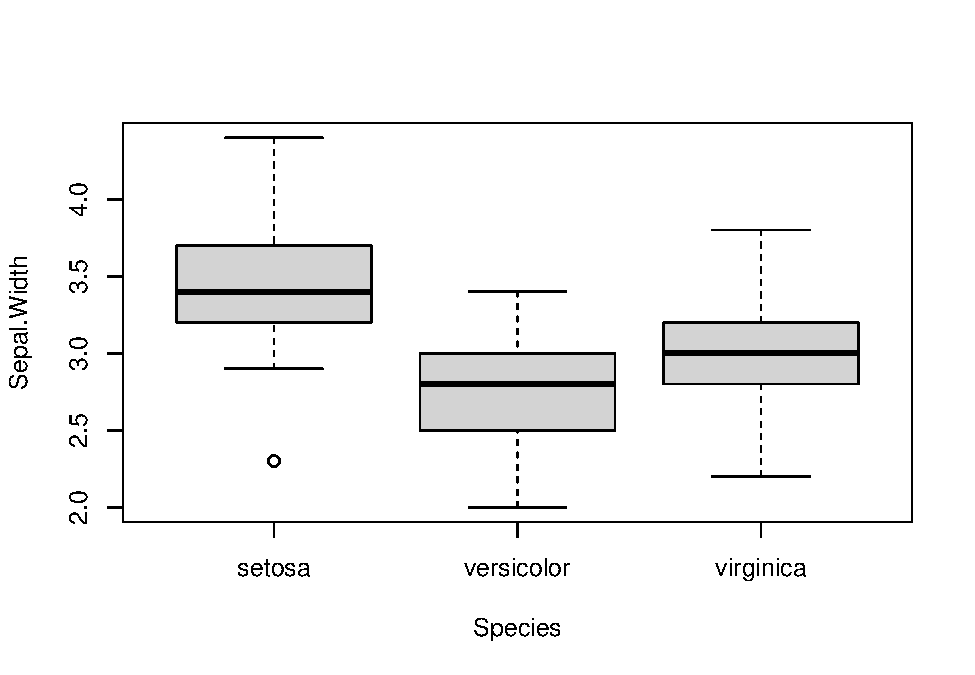
\includegraphics[keepaspectratio]{01_EYNTKBYLR_files/figure-latex/unnamed-chunk-37-1.pdf}}

\textbf{Step 6} - Develop it

Once you have a minimal viable product of what you want to create, now it is time to develop your code. This could mean, making plots look better, making analysis more sophisticated, or simply organising your code better for yourself or another reader.

For example, we might improve our code above by using the \texttt{ggplot2} package and adding in some comments for the user.

\begin{Shaded}
\begin{Highlighting}[]
\CommentTok{\# Load in ggplot packages}
\FunctionTok{library}\NormalTok{(ggplot2)}

\CommentTok{\# Plot a boxplot of sepal widths coloured by iris species}
\FunctionTok{ggplot}\NormalTok{(iris, }\FunctionTok{aes}\NormalTok{(}\AttributeTok{x =}\NormalTok{ Species, }\AttributeTok{y =}\NormalTok{ Sepal.Width, }\AttributeTok{fill =}\NormalTok{ Species)) }\SpecialCharTok{+}
  \FunctionTok{geom\_boxplot}\NormalTok{() }\SpecialCharTok{+}
  \FunctionTok{labs}\NormalTok{(}
    \AttributeTok{title =} \StringTok{"Sepal Width by Species"}\NormalTok{,}
    \AttributeTok{x =} \StringTok{"Species"}\NormalTok{,}
    \AttributeTok{y =} \StringTok{"Sepal Width"}
\NormalTok{  ) }\SpecialCharTok{+}
  \FunctionTok{theme\_minimal}\NormalTok{()}
\end{Highlighting}
\end{Shaded}

\pandocbounded{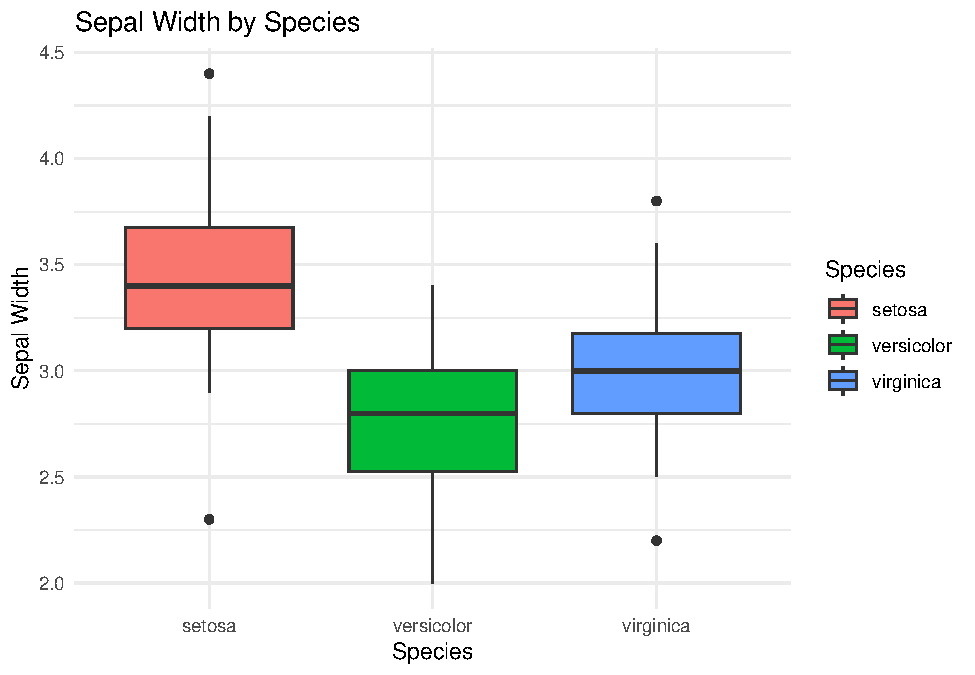
\includegraphics[keepaspectratio]{01_EYNTKBYLR_files/figure-latex/unnamed-chunk-38-1.pdf}}

\section{Final advice}\label{final-advice}

When learning R, you may sometimes feel that everyone else understands it except you.

That's not true.

Even experienced R users regularly search for functions, look at documentation, make mistakes and spend time figuring out why something isn't working.

The difference is that, with practice, you gradually become better at solving those problems.

You do not need to become an expert before you can use R.

You just need to keep building your knowledge.

\begin{quote}
\textbf{Start small. Practise often. Don't be afraid of errors. Ask for help.}
\end{quote}

\section{Your R learning checklist}\label{your-r-learning-checklist}

Use this checklist to keep track of your progress.

\begin{itemize}
\tightlist
\item[$\square$]
  I understand what R is.
\item[$\square$]
  I understand the difference between R and RStudio.
\item[$\square$]
  I have installed R.
\item[$\square$]
  I have installed RStudio.
\item[$\square$]
  I can open RStudio.
\item[$\square$]
  I know where to find the \href{https://sheffield.ac.uk/mash/stats-resources/r\#First-steps}{MASH First steps in R resources} page.
\item[$\square$]
  I know what the Console is.
\item[$\square$]
  I know what an R script is.
\item[$\square$]
  I understand the difference between the Console and a script.
\item[$\square$]
  I know what a command is.
\item[$\square$]
  I know what a function is.
\item[$\square$]
  I know what an argument is.
\item[$\square$]
  I can create an object.
\item[$\square$]
  I can create a vector.
\item[$\square$]
  I can call a function.
\item[$\square$]
  I know what a package is.
\item[$\square$]
  I know the difference between installing and loading a package.
\item[$\square$]
  I know how to find help for a function.
\item[$\square$]
  I understand what a working directory is.
\item[$\square$]
  I know how to save an R script.
\item[$\square$]
  I know how to \href{https://students.sheffield.ac.uk/mash/bookings/stats-support\#book-here}{book a MASH 1:1 appointment}.
\item[$\square$]
  I know how to \href{https://students.sheffield.ac.uk/mash/workshops\#bookig-calendar}{book a MASH R workshop}
\end{itemize}

\section{Glossary}\label{glossary}

\begin{longtable}[]{@{}
  >{\raggedright\arraybackslash}p{(\linewidth - 2\tabcolsep) * \real{0.5000}}
  >{\raggedright\arraybackslash}p{(\linewidth - 2\tabcolsep) * \real{0.5000}}@{}}
\toprule\noalign{}
\begin{minipage}[b]{\linewidth}\raggedright
Term
\end{minipage} & \begin{minipage}[b]{\linewidth}\raggedright
Brief description
\end{minipage} \\
\midrule\noalign{}
\endhead
\bottomrule\noalign{}
\endlastfoot
\textbf{R} & A programming language used for statistics, data analysis and data visualisation. \\
\textbf{RStudio} & An Integrated Development Environment (IDE) that provides an interface for working with R. \\
\textbf{Command} & An instruction given to R to perform an action. \\
\textbf{Function} & A piece of code designed to perform a particular task. \\
\textbf{Argument} & Information supplied to a function that tells it what to work with or how to behave. \\
\textbf{Object} & Something that R can store and work with, such as a number, text or vector. \\
\textbf{Assignment} & The process of storing a value in an object, commonly using \texttt{\textless{}-}. \\
\textbf{Package} & A collection of additional functions, data and resources that extends R's capabilities. \\
\textbf{Script} & A saved file containing R code, usually with the \texttt{.R} file extension. \\
\textbf{Console} & The RStudio pane where R commands are entered and executed. \\
\textbf{Source} & The RStudio pane where you write, edit and save R scripts. \\
\textbf{Environment} & The RStudio pane showing objects currently stored in your R session. \\
\textbf{History} & An RStudio tab showing commands previously entered during your session. \\
\textbf{Working directory} & The folder R uses as its default location for reading and writing files. \\
\textbf{Comment} & Text beginning with \texttt{\#} that R ignores when executing code. \\
\textbf{Debugging} & The process of finding and fixing problems in code. \\
\textbf{Error} & A message from R indicating that something has gone wrong when running code. \\
\textbf{Warning} & A message from R indicating that something may not have worked as expected. \\
\end{longtable}

\chapter{Downloading R and RStudio}\label{downloading-r-and-rstudio}

\section{Introduction}\label{introduction}

\begin{center}\rule{0.5\linewidth}{0.5pt}\end{center}

This is the first document in our ``First Steps in \textbf{\emph{R}}'' series of resources.

\textbf{\emph{R}} is a programming language specifically designed for doing statistics. The \textbf{\emph{R}} software can be downloaded on its own but it is more usual to download both \textbf{\emph{R}} and \textbf{\emph{RStudio}}. \textbf{\emph{RStudio}} is a more convenient way of interacting \textbf{\emph{R}}. The \textbf{\emph{R}} \emph{software} must be installed before \textbf{\emph{RStudio}} will work.

\section{\texorpdfstring{Downloading \textbf{\emph{R}} for Windows (do this first, before downloading \textbf{\emph{RStudio}})}{Downloading R for Windows (do this first, before downloading RStudio)}}\label{downloading-r-for-windows-do-this-first-before-downloading-rstudio}

\textbf{\emph{R}} can be downloaded from CRAN (the Comprehensive R Archive Network).

Click ``\textbf{Download R-4.4.1 for Windows}''.

Figure 1: The link to click to download R for Windows.

When the file has downloaded, open it just as you would when installing any other new program.

We would recommend you agree with the default settings and perhaps consider clicking the boxes to add a desktop shortcut and a \textbf{\emph{Quick Launch}} shortcut.

\section{\texorpdfstring{Downloading \textbf{\emph{R}} for other operating systems}{Downloading R for other operating systems}}\label{downloading-r-for-other-operating-systems}

Go to CRAN (the Comprehensive R Archive Network). Select the appropriate operating system from the options given then download the latest release from the following page.

Figure 2: The links to click to download R for other operating systems.

\section{\texorpdfstring{Downloading \textbf{\emph{RStudio}} (you will need to download \textbf{\emph{R}} first to enable \textbf{\emph{RStudio}} to work)}{Downloading RStudio (you will need to download R first to enable RStudio to work)}}\label{downloading-rstudio-you-will-need-to-download-r-first-to-enable-rstudio-to-work}

Go to R Studio.

Scroll down a little and choose the free version of \textbf{\emph{RStudio}} and click ``\textbf{Download}.''

Figure 3: The button to click to download RStudio.

Click ``\textbf{Download} \textbf{\emph{RStudio}} \textbf{for Windows}'' (or select your operating system from the list a little further down).

Again, open the file just as you would when installing any other new program and select the default options.

\chapter{First interactions with R and RStudio}\label{first-interactions-with-r-and-rstudio}

\section{Introduction}\label{introduction-1}

This document is part of our ``First Steps in \textbf{\emph{R}}'' resources. It is assumed that the reader has downloaded \textbf{\emph{R}} and \textbf{\emph{RStudio}}. No other pre-knowledge is required.

Most of the time we are used to interacting with a computer through a Graphical User Interface (GUI) (i.e.~with folders, files, windows etc). In \textbf{\emph{R}} and \textbf{\emph{RStudio}}, we type instructions (code) instead. The window the instructions are typed into is called the console. Of course, we must type our instructions in a way the computer will understand - this is why it's called a programming \emph{language}. This is the way computers were operated before the development of GUIs. \textbf{\emph{R}} is a programming language which has been developed specifically for doing statistics. \textbf{\emph{R}} and \textbf{\emph{RStudio}} are pieces of software which allow the computer to read the code we type and execute it (i.e.~follow the instructions).

\section{\texorpdfstring{Opening \textbf{\emph{R}}}{Opening R}}\label{opening-r}

If you open the \textbf{\emph{R}} software you will get a window in which you can type code. This is the console. It is possible to use the \textbf{\emph{R}} package to do statistics with \textbf{\emph{R}} but \textbf{\emph{RStudio}} is much more friendly to use. \textbf{\emph{RStudio}} is called an Integrated Development Environment (IDE) for \textbf{\emph{R}}. Note that for \textbf{\emph{RStudio}} to work, it requires that \textbf{\emph{R}} is also installed. Because of its ease of use, once you've used \textbf{\emph{RStudio}}, you will probably find you never open \textbf{\emph{R}} again! All of the materials in this series use \textbf{\emph{RStudio}} for this reason.

\section{\texorpdfstring{First Opening \textbf{\emph{RStudio}}}{First Opening RStudio}}\label{first-opening-rstudio}

When you open \textbf{\emph{RStudio}} for the first time there will be three windows. The one on the left is the console. You can type code directly in here and \textbf{\emph{RStudio}} will follow your instructions as soon as you press return. One thing \textbf{\emph{R}} can do is simple calculations like a calculator. You can experiment by typing calculations in the console. If you type 4+6 and press return, \textbf{\emph{R}} will give you the answer \(10\).

Figure 1: RStudio when it is opened for the first time.

If you'd like to carry out other calculations, here are the ways you must enter them into \textbf{\emph{RStudio}} for some simple operations.

\begin{longtable}[]{@{}cc@{}}
\toprule\noalign{}
Arithmetic Operation & R Code \\
\midrule\noalign{}
\endhead
\bottomrule\noalign{}
\endlastfoot
\(4+6\) & 4+6 \\
\(6-4\) & 6-4 \\
\(4 \times 6\) & 4*6 \\
\(4 \div 6\) & 4/6 \\
\(4^{6}\) & 4\^{}6 \\
\(\mathrm{e}^{4}\) & exp(4) \\
\(\log_{10} (4)\) & log10(4) \\
\(\ln(4)\) & log(4) \\
\end{longtable}

Note that you cannot go back and delete text you have put in the console. If you've never done any coding at first this may seem strange but you'll get used to it quickly.

\section{Inputting Code Using a Script}\label{inputting-code-using-a-script}

A Script is the name for some code that has been written and which we want \textbf{\emph{R}} to execute for us. You can write a script, edit it, save it then open it in \textbf{\emph{RStudio}} and run it whenever you like. \textbf{\emph{RStudio}} will let you let you edit your script until you're happy with it and then run all or just some of it by highlighting and clicking run. If you choose ``\textbf{Save As}\ldots{}'' in the file menu (as you would when saving, say, a \textbf{\emph{Word}} document) the script is what gets saved. To create a \textbf{Script file} for the first time, in \textbf{\emph{RStudio}}, click ``\textbf{File}'' then select ``\textbf{New File}'' and ``\textbf{R Script}.''

Figure 2: How to create a Script file in RStudio for the first time.

A fourth window opens up on the top left in \textbf{\emph{RStudio}}. Try typing a few calculations in here. You will see that \textbf{\emph{RStudio}} will let you type without carrying out any of the calculations. See what happens if you highlight the text and click ``\textbf{Run}.''

Figure 3: The fourth window, for scripts, in RStudio.

You should find that all the calculations are carried out at once in the console like so:

Figure 4: The calculations are carried out in the console in RStudio all at once when the script is run.

\section{The Environment}\label{the-environment}

As we write code, we will create ``\textbf{\emph{objects}}''. The word has a technical use in \textbf{\emph{R}} programming which we will deal with in future worksheets. For now we will think of an object as being similar to a variable in algebra - i.e.~a letter to which we can assign a value.

We can tell \textbf{\emph{R}} that we are creating a new object using the ``\textbf{\emph{assignment operator}}'':

\textless-

You can think of this as an arrow. The name of the new object should go on the left and the definition goes on the right. So the code

x \textless- 3

would create a new object called x which is defined to have the value \(3\). If we then type

x+4

We should find that \textbf{\emph{R}} calculates \(3+4\) and returns the answer \(7\).

Type

x \textless- 3

in the console then look in the top right window. You should find that it looks like this.

Figure 5: The top right window (the ``Environment'') in RStudio, where x is defined to have the value \(3\).

(Note: You can use = as an assignment operator as well as \textless-. However, there is a technical difference in the way \textbf{\emph{R}} reads =. In most situations, either = or \textless- can be used interchangeably but it is a good practice to stick to \textless- when defining a new object.)

When we are writing code we may want to define many new objects. These objects then exist in the \textbf{\emph{R}} ``Environment''. As we create new objects, the top right window keeps a record of them for us. This helps us keep track and can help us ensure that we do not create two objects with the same name.

We can ask \textbf{\emph{R}} to give us the same information by typing ls() in the console. ``ls'' is short for list - we are asking \textbf{\emph{R}} to list all the objects in the environment.

You can remove an object from the environment by typing

rm()

with the name of the object in the brackets.

For example,

rm(x)

would remove our variable x from the environment.

You can delete all objects from the environment by clicking the broom icon in the top ribbon of the ``Environment'' window:

Figure 6: How to delete all objects from the environment in RStudio.

Alternatively, you can type the following command in the console:

rm(list=ls())

(Note: we don't need to worry about the details of this command at the moment but in case you're interested: ``rm'' tells \textbf{\emph{R}} to remove the thing in the brackets. The rest of the code tells \textbf{\emph{R}} that it is going to remove an object which is a ``list'' and that list is called ls(). A ``list'' is a category of object in \textbf{\emph{R}}. ls() is specifically the list of everything in the environment.)

\section{The Bottom Right Window}\label{the-bottom-right-window}

There are several tabs in the window in the bottom right. For the moment we will only worry about two of them: ``Plots'' and ``Help''. If we ask \textbf{\emph{RStudio}} to draw a graph or chart, it will appear in this window under this tab. If we ask \textbf{\emph{RStudio}} for help - which we will often do when learning how to use a new piece of code - the answer will appear under the ``Help'' tab.

\section{Exercise}\label{exercise}

\begin{enumerate}
\def\labelenumi{\arabic{enumi}.}
\tightlist
\item
  In the console, create an object called y and give it the value \(15\).\\
\item
  Create another object called z and give it the value \(5\).\\
\item
  Calculate y divided by z.\\
\item
  Clear the environment and repeat the above by writing a script to do all three stages and running it.
\item
  Change the value of y in your script to \(20\) and run it again.
\end{enumerate}

\subsection{Solutions}\label{solutions}

Solutions

\begin{enumerate}
\def\labelenumi{\arabic{enumi}.}
\item
  \textgreater{} y \textless- 15
\item
  \textgreater{} z \textless- 5\\
  \textgreater{} y\\
  {[}1{]} 15\\
  \textgreater{} z\\
  {[}1{]} 5
\item
  \textgreater{} y/z\\
  {[}1{]} 3
\item
  Script:\\
  y \textless- 20\\
  z \textless- 5\\
  y\\
  z\\
  y/z\\
  And here it is run:\\
  \textgreater{} y \textless- 20\\
  \textgreater{} z \textless- 5\\
  \textgreater{} y\\
  {[}1{]} 20\\
  \textgreater{} z\\
  {[}1{]} 5\\
  \textgreater{} y/z\\
  {[}1{]} 4
\end{enumerate}

\chapter{Vectors}\label{vectors}

\section{Introduction}\label{introduction-2}

This document is part of our ``First Steps in \textbf{\emph{R}}'' resources. It is assumed that the reader has downloaded \textbf{\emph{R}} and \textbf{\emph{RStudio}} and is familiar with the idea of typing commands into the console. If you would like a reminder of these ideas, resources can be found on the MASH website.

John Chambers, one of the creators of the \textbf{\emph{R}} programming language, once said ``To understand computations in \textbf{\emph{R}}, two slogans are helpful: 1. Everything that exists is an object. 2. Everything that happens is a function call.'' Objects in \textbf{\emph{R}} come in various categories such as Vectors, Matrices, Data Frames and Lists. The simplest of these is vectors.

The word vector is used in different ways in different contexts. In \textbf{\emph{R}} we can think of a vector ``as a list of things in order'', similar to the idea of a vector in mathematics.

\section{Defining a Numerical Vector}\label{defining-a-numerical-vector}

To define a new object in \textbf{\emph{R}} we must give it a name. The name must be a continuous string of characters with no spaces. For example, if we wanted to define an object called ``New Vector'' sensible names would be

NewVector
new\_vector
new.vector

Once we have chosen a name for our new object, we need to assign it a value. We do this with the assignment operator

\textless-

So if we type

new\_vector \textless-

we have so far told \textbf{\emph{R}} that we are going to define a new object called new\_vector. What we type next will be the definition of the object. To define a vector we need to use the letter c for ``combine''. So the command

new\_vector \textless- c(2,4,6,8)

would be read by \textbf{\emph{R}} as ``combine the numbers \(2, 4, 6\) and \(8\) into a vector and give them the label new\_vector''. Note that the elements of a vector must be separated by commas as shown.

When typing code it is important to be precise. A single character out of place might make the code unreadable for the computer. However, \textbf{\emph{R}} will ignore spaces (unless they are in the middle of the name of the object). So \textbf{\emph{R}} would read all of the following identically:

new\_vector \textless- c(2,4,6,8)
new\_vector \textless- c( 2 , 4 , 6 , 8 )
new\_vector \textless-c(2,4 , 6 , 8)

Define an object called new\_vector as above and look what happened in the ``Environment'' window (top right). You should see that the vector has appeared in the environment as follows:

Figure 1: The top right window (the ``Environment'') in RStudio, where new\_vector is shown to be stored as a numerical vector.

``num'' means that the vector has been stored by \textbf{\emph{R}} as a numerical vector and \textbf{\emph{R}} is reading the elements of the vector as numbers; 1:4 means that \textbf{\emph{R}} has labelled the elements of the vector as first, second, third and fourth and the final part lists the elements of the vector.

We can now ask \textbf{\emph{R}} to show us the vector by typing in the console window:

new\_vector

\textbf{\emph{R}} will then display our vector like so:

Figure 2: new\_vector is shown in the console in RStudio.

The {[}1{]} means that the first entry on that line is the first element of the vector.

We can also carry out calculations with our vector. Type the following:

new\_vector +2

and \textbf{\emph{R}} will add \(2\) to each element of the vector like so:

Figure 3: \(2\) is added to each element of new\_vector in the console in RStudio.

\section{Vectors using ``:''}\label{vectors-using}

Type the following into the console

vec2 \textless- 1:100
vec2

The first line defines a new object called vec2 and the second line asks \textbf{\emph{R}} to display that object. You should see that vec2 is a vector which consists of the whole numbers from \(1\) to \(100\). Looking in the environment will confirm that \textbf{\emph{R}} has stored vec2 as a numerical vector:

Figure 4: The ``Environment'' window in RStudio where vec2 is shown to be stored as a numerical vector.

``:'' is a shortcut to create vectors like this. Experiment by typing the following commands into the console

2:16
5.6:14
3.9:10

\section{Character Vectors}\label{character-vectors}

A character vector is similar to a numerical vector but \textbf{\emph{R}} will interpret the elements as words rather than numbers. This might be helpful if, for example, we have some data about different people and we want to include a list of their names. We define a character vector just like a numerical vector but we must put each element of the vector in inverted commas in the definition. For example:

people \textless- c(``Ali'', ``Bertha'', ``Charlie'')

defines a character vector called people which would store the names Ali, Bertha and Charlie. If you type this into the console you will see the new object appear in the environment like so:

Figure 5: The top right window (the ``Environment'') in RStudio where people is shown to be stored as a character vector.

``chr'' shows that \textbf{\emph{R}} is interpreting people as a character vector. Note that we did not need to tell \textbf{\emph{R}} what sort of vector we were defining. Putting the elements in inverted commas was enough for \textbf{\emph{R}} to know that our vector was a character vector.

The elements of a character vector are called \textbf{strings}.

In \textbf{\emph{R}} '' can often be replaced by ' without noticing the difference. The usual convention is to use ``.

(For completeness: if, for some reason, you want to define a string which contains the character ``, you should use ' at the beginning and the end of the definition.)

You will sometimes see vectors referred to as \textbf{atomic vectors}, which means that they can only contain one type of data. For example, a vector can contain either numeric or character values but not both in the same vector. If we try to define a vector with some numbers and some character strings, \textbf{\emph{R}} will interpret the numbers as character strings.

\section{Exercise}\label{exercise-1}

\begin{enumerate}
\def\labelenumi{\arabic{enumi}.}
\tightlist
\item
  Define a new vector called vec3 which stores the numbers \(3\), \(4\), \(7\), \(9\), \(12\).
\item
  Predict what the following code will do:

  vec3*1:5

  Now type the code in the console and check your prediction.
\item
  Predict what the following code will do:

  vec3+1:3

  Now type the code in the console and check your prediction.
\item
  Create a character vector ice.cream which contains the names of your favourite flavours of ice cream.
\end{enumerate}

(Note that in question \(3\) we get an output along with the warning message. When \textbf{\emph{R}} runs out of values in the second vector, it starts again with the first element.)

\subsection{Solutions}\label{solutions-1}

Solutions

Here is the code used to do the above exercise:

\begin{enumerate}
\def\labelenumi{\arabic{enumi}.}
\item
  \textgreater{} vec3 \textless- c(3,4,7,9,12)\\
  \textgreater{} vec3\\
  {[}1{]} 3 4 7 9 12
\item
  \textgreater{} vec3*1:5\\
  {[}1{]} 3 8 21 36 60
\item
  \textgreater{} vec3+1:3\\
  {[}1{]} 4 6 10 10 14\\
  Warning message:\\
  In vec3 + 1:3 :\\
  longer object length is not a multiple of shorter object length
\item
  \textgreater{} ice.cream \textless- c(``vanilla'',``coffee'',``strawberry'')\\
  \textgreater{} ice.cream\\
  {[}1{]} ``vanilla'' ``coffee'' ``strawberry''
\end{enumerate}

Additional notes:\\
2. vec3\emph{1:5 multiplies the first element of vec3 by \(1\), the second element by \(2\) and so on.\\
3. vec3+1:3 adds \(1\) to the first element of vec3, \(2\) to the second element and \(3\) to the third element. Then }\textbf{R}* ``recycles'' the numbers 1:3 so the fourth number in the output comes from the fourth element of vec3 plus \(1\) (i.e.~\(9+1=10\))

\textless{}\details\textgreater{}

\chapter{Functions}\label{functions}

\section{Introduction}\label{introduction-3}

This document is part of our ``First Steps in \textbf{\emph{R}}'' resources. It is assumed that the reader knows how to define a vector in \textbf{\emph{R}}. Defining vectors is dealt with in the previous document in this series which can also be found on the MASH website.

\section{Doing Calculations with Functions}\label{doing-calculations-with-functions}

When we type a function into the console, we say we are \textbf{calling} the function. For our first example we will call the function ``mean''. This function calculates the mean of the numbers in a numerical vector. First, we will define a numerical vector, for example:

numbers \textless- c(5,23,4,6,3)

We can now call the function mean:

mean(numbers)

If we type these two lines of code into the console, \textbf{\emph{R}} will calculate the mean of the numbers in the vector:

Figure 1: The mean of numbers is outputted in the console in RStudio..

Alternatively, we can define the vector within the brackets of the function. For example:

mean(c(5,23,4,6,3))

would produce the same result as:

numbers \textless- c(5,23,4,6,3)
mean(numbers)

A few more simple functions are summarised below:

\begin{longtable}[]{@{}
  >{\centering\arraybackslash}p{(\linewidth - 2\tabcolsep) * \real{0.5000}}
  >{\centering\arraybackslash}p{(\linewidth - 2\tabcolsep) * \real{0.5000}}@{}}
\toprule\noalign{}
\begin{minipage}[b]{\linewidth}\centering
Function
\end{minipage} & \begin{minipage}[b]{\linewidth}\centering
Definition
\end{minipage} \\
\midrule\noalign{}
\endhead
\bottomrule\noalign{}
\endlastfoot
sd() & Finds the standard deviation of the numbers in the input vector \\
var() & Finds the variance of the numbers in the input vector \\
median() & Finds the median of the numbers in the input vector \\
max() & Finds the maximum of the numbers in the input vector \\
min() & Finds the minimum of the numbers in the input vector \\
summary() & Finds the five number summary and the mean of the numbers in the input vector \\
\end{longtable}

In \textbf{\emph{R}}, a function always has brackets after its name. Usually, we type arguments (inputs) into the brackets. The above functions all require a vector as an argument. How many arguments a function requires and what the arguments are depend on the function. The important principle is that we type the name of the function, then open brackets, then the arguments, then close brackets. If there is more than one argument, we separate the arguments using commas.

\section{Functions with Other Uses}\label{functions-with-other-uses}

All the functions described above carry out calculations. Functions can also be used to tell us about properties of an object. Perhaps the simplest example is the ``length'' function. This function tells us how many elements there are in a vector. For example,

length(numbers)

would return the value \(5\).

The ``class'' function can be used to tell us what kind of object we are dealing with. For example,

class(numbers)

returns the word ``numeric'' because numbers is a numeric vector.

\section{\texorpdfstring{Using Functions to Manipulate the \textbf{\emph{R}} Environment}{Using Functions to Manipulate the R Environment}}\label{using-functions-to-manipulate-the-r-environment}

We are used to manipulating a computer using menus, windows and a mouse. This is called a GUI (Graphic User Interface). Before the development of GUIs, computers were given instructions by the user typing into a console. In \textbf{\emph{RStudio}}, we can use the mouse and menus or type instructions into the console. You may prefer a combination of both approaches.

We will look at three examples of functions we can use to manipulate the \textbf{\emph{R}} environment.

First, ``remove'' or ``rm'' can be used to remove an object from the environment.

remove(numbers)
or
rm(numbers)

would remove the object numbers from the \textbf{\emph{R}} environment. remove and rm can be used interchangeably.

We can see a list of all the objects we have defined so far using the function

ls()

ls is an abbreviation of ``list''. This is an example of a function which doesn't require any arguments (i.e.~we don't type anything in the brackets).

The remove function can also be used to delete all objects in the environment like so:

rm(list=ls())

It is a good idea to use this command before starting a new project so that it doesn't get difficult to keep track of the objects which you have defined. Here the argument of the rm function is list=ls(). This tells \textbf{\emph{R}} to remove a list of objects and that the list to be removed is the list given by the function ls(). Clicking on the broom symbol in the top right window in \textbf{\emph{RStudio}} has the same effect as typing rm(list=ls()) in the console.

Figure 2: The top right window (the ``Environment'') and the broom symbol in RStudio.

Finally, we can use

q()

to close \textbf{\emph{RStudio}}. ``q'' stands for quit.

\section{Looking Up Functions}\label{looking-up-functions}

\textbf{\emph{R}} is a programming language. We can think of all the available functions as the vocabulary of the language. We are unlikely ever to know the details of every function in \textbf{\emph{R}} (just as we are unlikely ever to learn every word in the dictionary). A wide ``vocabulary'' will allow us to do more with our language but even a few words will get us somewhere. A reasonable goal is to memorise the details of some useful functions which we use regularly and then make sure that we know how to look up functions which we use less often or which we have forgotten.

Typing ? followed by the name of a function will bring up the details of the function in the ``Help'' tab of the bottom right window in \textbf{\emph{RStudio}}. If we type

?mean

into the console, the ``Help'' tab shows the following:

Figure 3: The ``Help'' tab of the bottom right window in RStudio when ?mean is typed into the console.

We see that we can input more than one argument into the mean function. We can, for example, use the mean function like so:

mean(vector, rm.na=TRUE)

The argument rm.na=TRUE must be separated from the first argument by a comma. rm.na is short for ``remove entries of NA from the vector before calculating the mean.'' ``NA'' is short for ``Not Available'' and it is the standard label for a missing piece of data in \textbf{\emph{R}}. rm.na is set to FALSE by default. In the example above we have set it to TRUE (so values of NA will be removed).

It often happens that when we use the ``Help'' tab to look up a function we have been using, we discover that we can use the function to do more than we thought. We may well find that we don't understand all the information given in the ``Help'' tab. Usually, we can find the information we need and not worry about other details.

If we suspect a function exists in \textbf{\emph{R}} but we don't know what it is, a Google search will often help. The MASH website has materials to help you get to grips with many functions for carrying out the most common statistical processes.

If we can't find a function which works the way we would like, we can define a new function using \textbf{\emph{R}}. The MASH website contains other resources to help you learn how to do this.

\section{Exercise}\label{exercise-2}

\begin{enumerate}
\def\labelenumi{\arabic{enumi}.}
\tightlist
\item
  Define a numerical vector with at least ten of your favourite numbers.
\item
  Use \textbf{\emph{R}} to find the mean, median and standard deviation of the numbers in your vector.
\item
  Remove your vector from the environment using a command in the console.
\item
  Check your vector has been removed by checking the list of all objects in the environment (do this by typing the appropriate command in the console).
\item
  Use the ``Help'' tab to look up the details of the ``median'' function.
\item
  Close \textbf{\emph{RStudio}} without touching your mouse.
\end{enumerate}

\subsection{Solutions}\label{solutions-2}

Solutions

Code used:

\begin{enumerate}
\def\labelenumi{\arabic{enumi}.}
\item
  \textgreater{} new\_vect \textless- sample(1:100,20, replace=TRUE)
\item
  \textgreater{} mean(new\_vect)\\
  {[}1{]} 48.95\\
  \textgreater{} median(new\_vect)\\
  {[}1{]} 48.5\\
  \textgreater{} sd(new\_vect)\\
  {[}1{]} 29.63191
\item
  \textgreater{} rm(new\_vect)
\item
  ls()
\item
  \textgreater{} ?median
\end{enumerate}

Notes:

The code

sample(1:100,20, replace=TRUE)

tells \textbf{\emph{R}} to sample \(20\) numbers at random from the vector 1:100 (i.e.~pick \(20\) numbers from \(1, 2, 3, \ldots , 100\) at random).

replace=TRUE

means that each number can be picked more than once.

You could also answer this question by picking the numbers yourself, e.g.:

new\_vect \textless- c(\ldots)

To close \textbf{\emph{RStudio}} without using your mouse, use the q() or type: \textbf{Ctrl+Q}.

\chapter{Matricies}\label{matricies}

\section{Introduction}\label{introduction-4}

This document is part of our ``First Steps in \textbf{\emph{R}}'' resources. It follows on from similar documents about vectors and functions in \textbf{\emph{R}}. It is assumed that the reader understands how to define numerical and character vectors and call a function in \textbf{\emph{R}}. If you would like to recap these topics, the documents and videos are on the MASH website.

\section{What is a Matrix?}\label{what-is-a-matrix}

In mathematics, a vector can be thought of as a single line of numbers in order, usually written in a column like so:

\[
\begin{bmatrix}
2 \\
1 \\
0 \\
7 \\
4 \\
\end{bmatrix}
\]

A matrix is a grid of numbers arranged in rows and columns like so:

\[
\begin{bmatrix}
2 & 1 & 0 & 5 \\
4 & 2 & 3 & 9 \\
0 & 8 & 8 & 1 \\
\end{bmatrix}
\]

Although there are differences between matrices in \textbf{\emph{R}} and in mathematics, this grid arrangement is the key feature that they have in common.

\section{\texorpdfstring{Defining a Numerical Matrix in \textbf{\emph{R}}}{Defining a Numerical Matrix in R}}\label{defining-a-numerical-matrix-in-r}

The following code is used to define a matrix in \textbf{\emph{R}}. We will look at the elements of the code in turn:

new\_matrix \textless- matrix(1:20, nrow=4, ncol=5)

In \textbf{\emph{R}}, a matrix is an ``object.'' To define any new object we begin by giving it a name. Then we use the assignment operator \textless- to tell \textbf{\emph{R}} that the definition of the object is about to follow. We will call our matrix ``new\_matrix'':

new\_matrix \textless-

So far, everything is the same as if we were defining a vector. Next we use the function ``matrix'' to tell \textbf{\emph{R}} that the object we are defining will be a matrix.

Once we have stated which numbers we want to arrange in a matrix, we next specify how many rows and columns we want the matrix to have.

In the above example, we chose \(4\) rows and \(5\) columns.

The first argument of the matrix function must be a vector. In the above example we have used the vector 1:20 which is just the numbers \(1\), \(2\), \(3\), \(\ldots\) , \(20\). Any vector can be used. The vector can be defined inside the matrix function like so:

new\_matrix2 \textless- matrix(c(2,3,2,3,4,6,3,7,6), nrow=3, ncol=3)

In the above example the code tells \textbf{\emph{R}} to concatenate (join together) the \(9\) numbers (\(2\), \(3\), \(2\), \(3\), \(4\), \(6\), \(3\), \(7\), \(6\)) into a matrix with \(3\) rows and \(3\) columns. Alternatively, we can define the vector first and use the name of the vector as an argument like so:

eg\_vector \textless- c(2,3,2,3,4,6,3,7,6)
new\_matrix2 \textless- matrix(eg\_vector, nrow=3, ncol=3)

If we define this matrix:

new\_matrix \textless- matrix(1:20, nrow=4, ncol=5)

in \textbf{\emph{R}} and then ask \textbf{\emph{R}} to show us the matrix (by typing new\_matrix) we get the following output:

Figure 1: new\_matrix, with the data from the vector 1:20 arranged by going down the first column, then the second column and so on, is shown in the console in RStudio.

By default \textbf{\emph{R}} arranges the data from our vector 1:20 by going down the first column, then the second column and so on. The matrix function has a fourth argument byrow which is set to FALSE by default. If we change byrow to TRUE, \textbf{\emph{R}} starts by assigning data to the first row, then the second row and so on:

Figure 2: new\_matrix, with the data from the vector 1:20 arranged by going along the first row, the second row and so on, is shown in the console in RStudio.

The preferred order for the arguments in the matrix function is as shown above. The vector containing the data must \textbf{always} be the first argument. However, we can put the other arguments in any order as long as the labels nrow=, ncol= and byrow= are used. Without labels, these arguments \textbf{must} be in the order shown above. Each of these three lines of code all define exactly the same matrix:

new\_matrix \textless- matrix(1:20, nrow=4, ncol=5, byrow=TRUE)
new\_matrix \textless- matrix(1:20, ncol=5, byrow=TRUE, nrow=4)
new\_matrix \textless- matrix(1:20, 4, 5, TRUE)

\section{Character Matrices}\label{character-matrices}

The previous examples discuss numerical matrices. If we define a character vector and ask \textbf{\emph{R}} to arrange it into a matrix, the resulting matrix is called a character matrix.

For example:

char\_vec = c(``a'', ``b'', ``c'', ``d'', ``e'', ``f'', ``g'', ``h'', ``i'')
char\_matrix \textless- matrix(char\_vec, nrow=3, ncol=3)
char\_matrix

produces the following:

Figure 3: char\_matrix is shown in the console in RStudio.

If we define char\_matrix and new\_matrix as above, we can see in the ``Environment'' window (top right) that the first is stored as a character matrix and the second as a numeric matrix.

Figure 4: The top right window (the ``Environment'') in RStudio where char\_matrix is shown to be a stored as a character matrix and new\_matrix is shown to be stored as a numeric matrix.

chr stands for character and int stands for integer (since all the numbers in our numeric matrix are integers).

\section{Combining Vectors to Make Matrices}\label{combining-vectors-to-make-matrices}

It may be more convenient to define a vector for each row or column of a matrix and then ask \textbf{\emph{R}} to put the vectors together into a matrix. This can be done with the rbind and cbind functions. rbind combines the vectors as rows and cbind as columns like so:

Figure 5: The vectors one, two and three are combined as rows and as columns to make matrices, outputted in the console in RStudio.

\section{Combining Numeric and Character Vectors}\label{combining-numeric-and-character-vectors}

Numeric and character vectors can be combined to make a matrix using rbind or cbind like so:

Figure 6: The vectors one and alpha are combined as rows to make the matrix eg, outputted in the console in RStudio.

But if we check how \textbf{\emph{R}} has stored this matrix, we will see that it is a character matrix:

Figure 7: The top right window (the ``Environment'') in RStudio where eg is shown to be stored as a character matrix.

This means that \textbf{\emph{R}} is now classifying the first row of the matrix as characters and not numbers. Matrices can only have one data type, and when we combine a character vector and a numeric vector, the numeric data is `coerced' to become characters. If we want a row (or column) of numerical data and another with data stored as characters, we need to use a data frame. Data frames are dealt with in other documents in this series which can be found on the MASH website.

\section{Exercise}\label{exercise-3}

In \textbf{\emph{RStudio}}, define:

\begin{enumerate}
\def\labelenumi{\arabic{enumi}.}
\tightlist
\item
  A numerical matrix ordered by columns
\item
  A numerical matrix ordered by rows
\item
  A character matrix
\item
  Three numerical vectors of length \(5\) called a, b and c
\item
  A matrix which has vectors a, b and c as rows
\item
  A matrix which has vectors a, b and c as columns
\end{enumerate}

\subsection{Solutions}\label{solutions-3}

Solutions

\begin{enumerate}
\def\labelenumi{\arabic{enumi}.}
\item
  First let's create a numerical vector of random integers using the sample() command. The following creates a vector of random integers between \(0\) and \(9\) of length \(12\):\\
  \textgreater{} num\_vect1 \textless- sample(0:9, 12,replace=TRUE)\\
  \textgreater{} num\_vect1\\
  {[}1{]} 1 6 1 1 7 5 3 2 7 5 9 0\\
  Now create a matrix ordered by columns (remember the default is by columns):\\
  \textgreater{} num\_mat\_col \textless- matrix(num\_vect1,nrow=3, ncol=4)\\
  \textgreater{} num\_mat\_col\\
  {[},1{]} {[},2{]} {[},3{]} {[},4{]}\\
  {[}1,{]} 1 1 3 5\\
  {[}2,{]} 6 7 2 9\\
  {[}3,{]} 1 5 7 0
\item
  Now create a matrix ordered by rows:\\
  \textgreater{} num\_mat\_row \textless- matrix(num\_vect1,nrow=3, ncol=4, byrow=TRUE)\\
  \textgreater{} num\_mat\_row\\
  {[},1{]} {[},2{]} {[},3{]} {[},4{]}\\
  {[}1,{]} 1 6 1 1\\
  {[}2,{]} 7 5 3 2\\
  {[}3,{]} 7 5 9 0
\item
  To create a sequential vector of letters, we can use either letters or LETTERS depending on whether you want lowercase or capitals. The following creates a character vector with the first \(12\) letters of the alphabet:\\
  \textgreater{} char\_vect \textless- letters{[}1:12{]}\\
  You can also take a random sample of letters of the alphabet using the sample() function:\\
  \textgreater{} char\_vect \textless- sample(1etters{[}1:12{]},12, replace=TRUE)\\
  \textgreater{} char\_vect\\
  {[}1{]} ``d'' ``a'' ``g'' ``d'' ``b'' ``f'' ``d'' ``f'' ``f'' ``b'' ``f'' ``i''\\
  The following uses the character vector that has been created to create a character matrix:\\
  \textgreater{} matrix\_char \textless- matrix(char\_vect,3,4)\\
  \textgreater{} matrix\_char\\
  {[},1{]} {[},2{]} {[},3{]} {[},4{]}\\
  {[}1,{]} ``d'' ``d'' ``d'' ``b'' \\
  {[}2,{]} ``a'' ``b'' ``f'' ``f'' \\
  {[}3,{]} ``g'' ``f'' ``f'' ``i'' \\
  Alternatively, you can pick the character strings for your matrix by hand:
  char\_vect \textless- c(``first word'', ``second word'', \ldots)
\item
  Now to create three vectors:\\
  \textgreater{} a \textless- sample(0:9,5,replace=TRUE)\\
  \textgreater{} b \textless- sample(0:9,5,replace=TRUE)\\
  \textgreater{} c \textless- sample(0:9,5,replace=TRUE)\\
  \textgreater{} a\\
  {[}1{]} 3 7 8 9 7\\
  \textgreater{} b\\
  {[}1{]} 7 2 9 7 3\\
  \textgreater{} c\\
  {[}1{]} 3 8 9 4 8\\
  (Again, these vectors have been produced by picking numbers between \(0\) and \(9\) at random. You don't have to use the same method here, any numbers will do in your vectors.)
\item
  \textgreater{} row\_matrix \textless- rbind(a,b,c)\\
  \textgreater{} row\_matrix\\
  {[},1{]} {[},2{]} {[},3{]} {[},4{]} {[},5{]}\\
  a 3 7 8 9 7\\
  b 7 2 9 7 3\\
  c 3 8 9 4 8
\item
  \textgreater{} col\_matrix \textless- cbind(a,b,c)\\
  \textgreater{} col\_matrix\\
  a b c\\
  {[}1,{]} 3 7 3\\
  {[}2,{]} 7 2 8\\
  {[}3,{]} 8 9 9\\
  {[}4,{]} 9 7 4\\
  {[}5,{]} 7 3 8
\end{enumerate}

\textless{}\details\textgreater{}

\chapter{Dataframes}\label{dataframes}

\section{Introduction}\label{introduction-5}

This document is part of our ``First Steps in \textbf{\emph{R}}'' resources. It follows on from similar documents about vectors, matrices and functions in \textbf{\emph{R}}. It is assumed that the reader understands how to define vectors and matrices and call a function in \textbf{\emph{R}}. If you would like to recap these topics, the documents and videos are on the MASH website.

\section{What is a Data Frame?}\label{what-is-a-data-frame}

A data frame is the name given in \textbf{\emph{R}} to a very common way of setting out data. The sampling units are arranged in rows and the variables in columns like so:

\begin{longtable}[]{@{}lccc@{}}
\toprule\noalign{}
& Physics score (\%) & Chemistry score (\%) & Hair Colour \\
\midrule\noalign{}
\endhead
\bottomrule\noalign{}
\endlastfoot
Alfred & 75 & 69 & Brown \\
Beatrice & 80 & 74 & Brown \\
Carl & 72 & 80 & Blonde \\
Daphne & 79 & 80 & Black \\
Earl & 65 & 70 & Blonde \\
\end{longtable}

This data frame records the scores in Physics and Chemistry along with the hair colour for five (fictional) people.

\section{\texorpdfstring{Defining a Data Frame in \textbf{\emph{R}}}{Defining a Data Frame in R}}\label{defining-a-data-frame-in-r}

Unlike a matrix, a data frame in \textbf{\emph{R}} can contain character and numeric data in different columns. However, each column must have either character or numeric data only.

A data frame is an object so creating one in \textbf{\emph{R}} is similar to creating a vector or matrix. In this case we use the function data.frame. The data.frame function takes vectors as arguments. These vectors form the columns of the data frame and the names of the vectors become the names of the columns. Remember, the columns in the data frame represent the variables, thus each vector contains the data for a single variable.

The following code defines a vector for each variable in the table above, combines the three vectors into a data frame and asks \textbf{\emph{R}} to show the data frame.

phys \textless- c(75,80,72,79,65)
chem \textless- c(69,74,80,80,70)
hair \textless- c(``Brown'', ``Brown'', ``Blonde'', ``Black'', ``Blonde'')
eg\_frame \textless- data.frame(phys, chem, hair)
eg\_frame

This is the result when we type this code into the console:

Figure 1: The vectors phys, chem and hair are combined to make the data frame eg\_frame, outputted in the console in RStudio.

\section{Setting the Row Names}\label{setting-the-row-names}

If we also want to record the names of the people in our survey, we could just add in another column with their names like so:

Figure 2: Another column, people, is added to the data frame eg\_frame, outputted in the console in RStudio.

But here, \textbf{\emph{R}} sees the people column as another variable we have recorded. If we want to tell \textbf{\emph{R}} that this column is special because it contains the names of our sampling units we need to label it using row.names.

We can do this in the definition of the data frame like so:

eg\_frame \textless- data.frame(phys, chem, hair, row.names = people)

or we can define the data frame as before and then use row.names as a function like so:

eg\_frame \textless- data.frame(phys, chem, hair)
row.names(eg\_frame) \textless- c(``Alfred'', ``Beatrice'', ``Carl'', ``Daphne'', ``Earl'')

With row names added by either of these methods, the data frame looks like this:

Figure 3: Row names are added to the data frame eg\_frame, outputted in the console in RStudio.

\section{Adding Extra Columns}\label{adding-extra-columns}

For the data frame above we can add a new column like so:

biology\_scores \textless- c(80, 69, 71, 72, 75)
eg\_frame\$bio \textless- biology\_scores

The first line defines a new vector called biology\_scores which contains the data we want to add to our data frame. The second line uses \$ to define a new column within the eg\_frame data frame called bio. This new column is then assigned the values from the vector biology\_scores.

Once the new column has been added, the data frame looks like this:

Figure 4: A new column, bio, is added to the eg\_frame data frame, outputted in the console in RStudio.

In general, to add a new column, we need code along these lines:

Name of data frame \$ name of new column \textless- vector containing data for the new column

\section{Exercise}\label{exercise-4}

1. Create a data frame in \textbf{\emph{R}} to record what you had for breakfast and how long it took you to travel to work/lectures each day last week (you can make up this data if you neglected to keep records). Set the row names as the days of the week when defining the data frame.\\
2. Record how long it took you to get home each day in a numeric vector (again, fictional data is acceptable). Add this vector to your data frame as a new column.\\
3. Create a data frame in \textbf{\emph{R}} containing the numbers in this table

\begin{longtable}[]{@{}cc@{}}
\toprule\noalign{}
Team 1 Score & Team 2 Score \\
\midrule\noalign{}
\endhead
\bottomrule\noalign{}
\endlastfoot
2 & 1 \\
1 & 1 \\
3 & 2 \\
2 & 4 \\
1 & 3 \\
\end{longtable}

4. Create a character vector containing the words game1, game2, game3, game4 and game5. Add this vector to your data frame as the row names.

\subsection{Solutions}\label{solutions-4}

Solutions

\begin{enumerate}
\def\labelenumi{\arabic{enumi}.}
\item
  \textgreater{} breakfast \textless- c(``egg'', ``toast'', ``toast'', ``cereal'', ``egg'')\\
  \textgreater{} am \textless- c(20,24,18,20,22)\\
  \textgreater{} days \textless- c(``Mon'', ``Tues'', ``Wed'', ``Thur'', ``Fri'')\\
  \textgreater{} Mornings \textless- data.frame(breakfast,am,row.names=days)\\
  \textgreater{} Mornings\\
  breakfast am\\
  Mon egg 20\\
  Tues toast 24\\
  Wed toast 18\\
  Thur cereal 20\\
  Fri egg 22
\item
  \textgreater{} pm \textless- c(23,26,24,28,20)\\
  \textgreater{} Mornings\$pm \textless- pm\\
  \textgreater{} Mornings\\
  breakfast am pm\\
  Mon egg 20 23\\
  Tues toast 24 26\\
  Wed toast 18 24\\
  Thur cereal 20 28\\
  Fri egg 22 20
\item
  \textgreater{} Team1Score \textless- c(2,1,3,2,1)\\
  \textgreater{} Team2Score \textless- c(1,1,2,4,3)\\
  \textgreater{} Scores \textless- data.frame(Team1Score,Team2Score)
\item
  \textgreater{} Games \textless- c(``game1'', ``game2'', ``game3'', ``game4'', ``game5'')\\
  \textgreater{} row.names(Scores) \textless- Games\\
  \textgreater{} Scores\\
  Team1Score Team2Score\\
  game1 2 1\\
  game2 1 1\\
  game3 3 2\\
  game4 2 4\\
  game5 1 3
\end{enumerate}

\chapter{Other objects}\label{other-objects}

\section{Introduction}\label{introduction-6}

This document is part of our ``First Steps in \textbf{\emph{R}}'' resources. In previous documents we discussed character and numeric vectors, matrices and data frames. It is assumed the reader is familiar with these topics. If you would like a recap, the materials are available on the MASH website. This document introduces the reader to some more commonly used kinds of object. If you are new to \textbf{\emph{R}}, it is not necessary to know all the details of every object available but it is useful to know that they exist.

\section{Factors}\label{factors}

A factor is useful for storing categorical data. A factor is similar to a vector but \textbf{\emph{R}} also keeps track of the ``levels'' of data. For example, if we are recording whether people are left or right handed, we might store our data in a vector like so:

handed \textless- c(``right'', ``left'', ``left'', ``right'', ``right'', ``right'', ``right'')

If we turn this data into a factor like so

eg\_factor \textless- factor(handed)

We find that when we ask \textbf{\emph{R}} to show us the object eg\_factor we get:

Figure 1: eg\_factor, with the levels of data, is shown in the console in RStudio.

The levels of data are left and right and this information is now also stored. We might need to use factors rather than character vectors because some functions expect data to be stored as a factor.

\section{Lists}\label{lists}

Vectors in \textbf{\emph{R}} contain a ``list'' of values. Separately, a list is also a kind of object in \textbf{\emph{R}}. A list-object can contain vectors, matrices, numbers, strings, data frames or anything else we can define as an object in \textbf{\emph{R}}. To define a list we use the command list() and the objects we wish to put in the list go in the brackets separated by commas.

If we create several diverse objects like so:

x \textless- c(4,2,5,3,6)
y \textless- matrix(1:20,4,5)
z \textless- 8*7
a \textless- c(``this'', ``is'', ``a'', ``character'', ``vector'')

We can then store them in a list like so:

eg\_list \textless- list (x,y,z,a)

When we ask \textbf{\emph{R}} to show us this list, we get the following:

Figure 2: The objects x, y, z and a are stored in the list eg\_list, outputted in the console in RStudio.

\section{Logical Vectors}\label{logical-vectors}

We have seen numeric and character vectors in previous documents. A third option is logical vectors. Logical values are TRUE and FALSE. \textbf{\emph{R}} associates a numerical value of \(1\) with TRUE and \(0\) with FALSE.

Logical vectors are usually used to consider the properties of other vectors.

For example, if we define a vector x as \(1, 2, 3, \ldots, 10\) like so:

x \textless- 1:10

Then the command

x \textgreater{} 5

asks \textbf{\emph{R}} to evaluate the statement x \textgreater{} 5 for each element of the vector x. A logical vector is returned like so:

Figure 3: The statement x \textgreater{} 5 is evaluated for each element of the vector x, and a logical vector is outputted in the console in RStudio.

A useful command is:

is.na(vector\_name\_here)

which can be used like so:

Figure 4: Each element of the vector vector is determined if it has the value NA and a logical vector is outputted in the console in RStudio.

The command

anyNA(vector\_name\_here)

will return a single result that is TRUE if a vector contains one or more value of NA and FALSE if there are no missing values in the vector.

\section{Arrays}\label{arrays}

A matrix can be thought of as a \(2\)-dimensional ``grid'' of numbers (or character strings) like so:

\[ \begin{array}{|c|c|c|c|}
\hline
2 & 4 & 1 & -5 \\ \hline
2 & 0 & 2 & 10 \\ \hline
-8 & -1 & 6 & 8 \\ \hline
0 & -6 & -7 & 9 \\ \hline
3 & 21 & 4 & 8 \\ \hline
\end{array}  \]

An array is the same as a matrix except we can have more than \(2\) dimensions. For example, we can picture a \(3\)-dimensional array like the cube below. We would have one value in each of the small cubes:

Figure 5: A cube representing a \(3\)-dimensional array.

In \textbf{\emph{R}} we can define an array like so:

array\_name \textless- array (data, dim = dimensions)

Here data is a vector containing the values to be put into the array and dimensions is a vector containing the dimensions of the array.

Example: If we wish to arrange the numbers \(1\) to \(27\) into a \(3 \times 3 \times 3\) cube we can do so thus:

eg\_array \textless- array(1:27, dim = c(3,3,3))

\textbf{\emph{R}} displays the array by showing one ``layer'' of the cube at a time like so:

Figure 6: The array eg\_array is outputted in the console in RStudio.

\chapter{Packages}\label{packages}

\section{Introduction}\label{introduction-7}

This document is part of our ``First Steps in \textbf{\emph{R}}'' resources. It is assumed that the reader has installed \textbf{\emph{R}} and \textbf{\emph{RStudio}} and understands how to type commands in the console. If you would like to recap these topics, the documents and videos are on the MASH website.

\section{What is a Package?}\label{what-is-a-package}

\textbf{\emph{R}} is a collaborative language, a little like Wikipedia. Anyone can write new functions or create new objects and make them available for other \textbf{\emph{R}} users in a package. You can think of a package like an app for a smartphone. Which packages you download will depend on what you want to do in \textbf{\emph{R}}. There are two ways of installing packages, either using menus or in the console window using \textbf{\emph{R}} commands.

\section{Installing Packages from Menus}\label{installing-packages-from-menus}

In the bottom right window of \textbf{\emph{RStudio}}, click on the ``\textbf{Packages}'' tab. In this tab you can see a list of all the packages which are already installed.

Figure 1: The ``Packages'' tab in the bottom right window in RStudio.

To install a new package that is not in the list, click ``Install'', which opens up the ``Install Packages'' dialogue box and allows you to download packages from the CRAN repository. CRAN stands for ``Comprehensive R Archive Network.'' This is a website which stores \textbf{\emph{R}} packages for \textbf{\emph{R}} users to download. You can think of it as the \textbf{\emph{R}} version of the App store on a smartphone.

Figure 2: The ``Install'' button in the ``Packages'' tab in the bottom right window in RStudio.

Type the name of the package you want to install. In this case we will install the package ggplot2. This is an often-recommended package which contains functions for making elegant graphs and charts.

Figure 3: The ``Install Packages'' dialogue box in RStudio.

When we click ``\textbf{Install}'' we will see the progress of the installation in the console. Depending on the package, the installation can take a few minutes. When the installation is finished we will receive a confirmation message in the console.

Our new package should now appear in the list of packages in the ``Packages'' tab.

Figure 4: The list of packages, with ggplot2 added, in the ``Packages'' tab in RStudio.

\section{Installing Packages Using the Console}\label{installing-packages-using-the-console}

The command install.packages() can be used to perform the same operation as described above. The name of the package to install should be in inverted commas like so:

install.packages(``ggplot2'')

\section{Using Your New Package}\label{using-your-new-package}

Once a package has been installed in \textbf{\emph{R}}, you will then need to tell \textbf{\emph{R}} that you want to use it. In the list of packages you will notice that some packages have a tick while most do not. The package we have just installed, ggplot2, does not have a tick. This means that the package has been downloaded (installed) but \textbf{\emph{RStudio}} is not interacting with it.

Figure 5: The empty box next to ggplot2 in the ``Packages'' tab in RStudio.

If we want to use the functions or objects from the new package we need to tell \textbf{\emph{R}} to access it using the library command like so:

library(ggplot2)

The functions and objects in the new package are now available to use and a tick has appeared in the list of packages.

Alternatively, we can find the package in the list of packages and tick the box using the mouse. You will notice that the library() command appears in the console window.

\chapter{Exploring Data}\label{exploring-data}

\section{Introduction}\label{introduction-8}

This document is part of our ``First Steps in \textbf{\emph{R}}'' resources. It is assumed that the reader understands the idea of an object, a function and a package in \textbf{\emph{R}}. If you would like to recap these topics, the documents and videos are on the MASH website.

\section{Built-in Datasets}\label{built-in-datasets}

When \textbf{\emph{R}} and \textbf{\emph{RStudio}} are first installed, several useful packages are installed by default. Two packages in particular contain datasets which are often used for exercises while learning \textbf{\emph{R}}. The ``datasets'' package containing \(104\) datasets is one that is already loaded. This means that all of its datasets are available immediately. To view information on the datasets package type the following into the \textbf{\emph{R}} console:

library(help=``datasets'')

This will give you brief details of the datasets including the name of each and a short description.

The command

data()

will produce a list of the datasets in the datasets package.

A second useful package, ``MASS'', contains \(87\) datasets. It is not loaded by default so to access its datasets we must first load the package using the command

library(MASS)

\section{Viewing a Dataset}\label{viewing-a-dataset}

``mtcars'' is a dataset contained in the datasets package. We will use this dataset as an example for the rest of this document. Like other datasets in the above packages, it is stored as a data frame in \textbf{\emph{R}}. Therefore we can view the data by simply typing

mtcars

into the console.

Figure 1: The mtcars data frame is shown in the console in RStudio.

We can find the details of what data is collected and how it is recorded using

?mtcars

The ``Help'' window then shows us the following:

Figure 2: The ``Help'' tab of the bottom right window in RStudio when ?mtcars is typed into the console.

If we want to access one variable from a dataset, we can use ``\$''. For example,

mtcars\$cyl

tells \textbf{\emph{R}} to look at the mtcars data frame and then find the variable labelled ``cyl''.

Figure 3: The data in the cyl column of the mtcars data frame is shown in the console in RStudio.

\section{Attaching the Dataset}\label{attaching-the-dataset}

If we are going to work with a dataset a lot we can use the ``attach'' command like so

attach(mtcars)

Once a dataset is attached, the variables can be accessed without needing to use the mtcars\$ prefix:

Figure 4: By attaching the mtcars dataset, the data in the cyl column of the mtcars data frame is shown in the console in RStudio.

Once you have finished working with the dataset, it is good practice to ``detach'' like so:

detach(mtcars)

\section{Functions For Getting to Know a Dataset}\label{functions-for-getting-to-know-a-dataset}

We can display a full dataset by simply typing the name of the data frame in which it is stored. However, a dataset may be too large to get a feel for the data this way. The following functions are useful for getting to know a dataset:

names()

gives a list of all the column names in the data frame.

Figure 5: A list of all the column names of the mtcars data frame is shown in the console in RStudio.

dim()

gives the number of rows and columns (in that order).

Figure 6: The number of rows and columns of the mtcars data frame is outputted in the console in RStudio.

In this example you can see that there are \(32\) rows and \(11\) variables in the data frame.

nrow() and ncol() can also be used for just the numbers of rows and/or columns.

head()

gives the first few rows of the data frame.

Figure 7: The first six rows of the mtcars data frame are outputted in the console in RStudio.

tail() is similar to head() but gives the last few rows.

str()

stands for ``structure''. This gives the number of observations and variables (rows and columns) followed by the name, data type of each column (numerical vector, character vector, logical vector or factor) and the first few entries in each variable:

Figure 8: The structure of the mtcars data frame is detailed in the console in RStudio.

``num'' is short for numerical. All the variables in this particular data frame happen to be numerical vectors.

summary()

gives a summary of each variable in the dataset.

Figure 9: A summary of each variable in themtcars dataset is outputted in the console in RStudio.

A column which stores a numeric vector gets summarised as above. A column which is stored in \textbf{\emph{R}} as a factor is summarised with how many times each level appears in the column. To see this try investigating the dataset ``esoph'' which is part of the dataset package. Hint: type ?esoph to see what data are stored in the dataset then str(esoph) to see which columns are numeric vectors and which are factors. Finally type summary(esoph) to see what the summary of a factor looks like.

\section{Exercise}\label{exercise-5}

\begin{enumerate}
\def\labelenumi{\arabic{enumi}.}
\tightlist
\item
  Use the data() command in the console to view a list of available datasets.\\
  Choose a dataset from the list and find out the following information:\\
\end{enumerate}

\begin{enumerate}
\def\labelenumi{\alph{enumi})}
\tightlist
\item
  What data are stored in the dataset\\
\item
  How many sampling units and how many variables there are\\
\item
  What type of variables the dataset contains (numeric, factor etc)\\
\item
  The maximum and minimum values of any numeric variables
\end{enumerate}

\subsection{Solutions}\label{solutions-5}

Solutions

\begin{enumerate}
\def\labelenumi{\arabic{enumi}.}
\tightlist
\item
  Initially I chose ``InsectSprays''.\\
\end{enumerate}

\begin{enumerate}
\def\labelenumi{\alph{enumi})}
\tightlist
\item
  I typed ?InsectSprays and the following information was displayed in the ``Help'' window (bottom right):\\

  Figure 10: The ``Help'' tab of the bottom right window in RStudio when ?InsectSprays is typed into the console.
\item
  There are two variables in the dataset and \(72\) observations/sampling units.\\
\item
  The first variable is numeric and contains the insect count. The second variable is a factor that codes for the type of insect spray that was used. At this point there is no information on the number of levels of the factor, but the usefulness of using the command ?InsectSprays is that the ``Help'' window gives you additional information such as the source of the dataset and a description of it.
\end{enumerate}

I then typed str(InsectSprays) to obtain the following info in the console window, which includes information on the number of level of the factor variable.

Figure 11: The structure of the InsectSprays data frame is detailed in the console in RStudio.

\begin{enumerate}
\def\labelenumi{\alph{enumi})}
\setcounter{enumi}{3}
\tightlist
\item
  There is only one numeric variable in this dataset so could type summary(InsectSprays\$count) to get only the info for this variable:
\end{enumerate}

Figure 12: Some summary statistics for the ``count'' variable in the InsectSprays dataset are outputted in the console in RStudio.

Alternatively, could simply type summary(InsectSprays) and get the information for all variables:

Figure 13: Some summary statistics for all variables in the InsectSprays dataset are outputted in the console in RStudio.

\chapter{Importing Data}\label{importing-data}

\section{Introduction}\label{introduction-9}

This document is part of our ``First Steps in \textbf{\emph{R}}'' resources. It is assumed that the reader understands how to define objects and call a function in \textbf{\emph{R}}. If you would like to recap these topics, the documents and videos are on the MASH website.

This document provides a guide to some of the ways to import a dataset to \textbf{\emph{R}}. It is by no means exhaustive! Users who are new to \textbf{\emph{R}} may wish to use the suggested method below and read no further.

\section{Preparing Data}\label{preparing-data}

It is sensible to ensure the data is well prepared to avoid any issues with reading data into \textbf{\emph{R}}.

In this document, we will be reading data from an Excel file. Before importing the data to \textbf{\emph{R}}, we must make sure that it is recorded in a way which will make it easy for \textbf{\emph{R}} to read.

Here are some useful practices:

\begin{itemize}
\tightlist
\item
  Use short names for variables and sampling units
\item
  Avoid names with symbols such as ?, \$, \%, \^{}, \&, *, (, ), -, /, \#, I, {[}, {]}, \{ and \}.
\item
  Avoid names, values and fields with blank spaces as they will be interpreted as separate variables, resulting in errors.
\item
  Use . or \_ to link words together if you need to, for example gene.length or gene\_length.
\item
  Do not make any comments in the Excel file. This will result in extra columns or NAs.
\item
  Replace missing values with NA. R recognises NA as missing data but \textbf{\emph{R}} would not recognise (for example) n/a as missing data.
\end{itemize}

\section{Importing the Data - Suggested Method}\label{importing-the-data---suggested-method}

This section focusses on one method for importing an Excel file, which I found easy to use when getting to know \textbf{\emph{RStudio}}. You may prefer to stick to this method, at least until you are more familiar with \textbf{\emph{R}}. Data can be imported to \textbf{\emph{R}} in various ways from various different pieces of software and other possibilities are discussed at the end of this document.

In the examples we will use the ``Birthweight'' dataset which can be found at MASH. The reader can follow the methods described with any Excel dataset.

Whichever file you decide to use, before importing into \textbf{\emph{R}}, save it as .txt (as tab-delimited text file) or .csv (comma delimited). To do this in Excel, just select the required file type when saving. In the examples we will use .csv.

Figure 1: The .txt and .csv file type options when saving Excel files.

Next, we type the following into the console:

birthweight \textless- read.csv(file.choose())

This code allows us to browse for the file on the computer. The first part tells \textbf{\emph{R}} that we are going to define a new object called ``birthweight'' (we could choose any name). Next we say that the definition of the object comes from the command ``read.csv''. This tells \textbf{\emph{R}} to create a data frame from the .csv file we are about to describe. The argument of the read.csv function is another function, ``file.choose''. This function will open a window which allows you to browse your folders and select the file you want. Note: the window sometimes opens \textbf{behind} the \textbf{\emph{RStudio}} window leaving the user to wonder where on earth it is!

Figure 2: The `Select file' window for browsing folders and files when using the file.choose() function as the argument of the read.csv function in RStudio.

Navigate to the folder where the file is, select the file and click ``\textbf{Open}''.

The dataset has now been imported to \textbf{\emph{R}} as a data frame. In the example, the data frame is called birthweight.

If the file is saved as a .txt instead of a .csv the above instructions can be followed using read.delim in place of read.csv.

\section{Typing a File Path}\label{typing-a-file-path}

The file path of the file can be typed directly into the read.csv function but you must remember:

\begin{itemize}
\tightlist
\item
  Put the file path in inverted commas ``file path\ldots{}''.
\item
  Replace each ``\(\backslash\)'' with ``\(\backslash \backslash\)''.
\item
  The name of the file must end .csv.
\end{itemize}

So a .csv file at this location:

C:\Users\User Name\Documents\Example folder\Birthweight\_reduced\_R

can be read into \textbf{\emph{R}} as a data frame called ``test'' using this command:

test \textless- read.csv(``C:\textbackslash Users\textbackslash User Name\textbackslash Documents\textbackslash Example folder\textbackslash Birthweight\_reduced\_R.csv'')

Note that unless the file is in the working directory (see below) the file.choose() function is usually an easier option.

\section{Importing a File Using the Menus}\label{importing-a-file-using-the-menus}

One final method for reading a file in is to use the menus. Files with the format .csv can be imported from menus by using the file browser tab in the bottom right window to browse to the file you want, then click on the file name and select ``\textbf{Import Dataset}'':

Figure 3: The bottom right window in RStudio, where files can be browsed and imported.

Alternatively, you can go to \textbf{File -\textgreater{} Import Dataset} to import .txt files or to import directly from Excel or SPSS (although you may need to install extra packages).

\section{The Working Directory}\label{the-working-directory}

\textbf{\emph{R}} has a location where it will save files to and import data from by default. This is referred to as the working directory. You can query what \textbf{\emph{R}} currently considers its working directory by running the command

getwd()

If a file is in the working directory and saved as a .csv then it can be imported to \textbf{\emph{R}} as a data frame like so:

Name of data frame here\textless- read.csv(``Type file name here'')

Remember to include .csv in the file name. Files in this directory can be listed using the function:

list.files()

And the working directory can be changed like so:

setwd(``Type file path here'')

But remember to replace ``\(\backslash\)'' with ``\(\backslash \backslash\)'' in the file path. Alternatively, the menus can be used by going to \textbf{Session -\textgreater{} Set Working Directory -\textgreater{} Choose Directory\ldots{}}

Figure 4: How to use the menus in RStudio to change the working directory for the rest of the session.

The new working directory is now set for the rest of the session. To change the working directory permanently, go to \textbf{Tools -\textgreater{} Global Options\ldots{}}

Figure 5: How to use the menus in RStudio to change the working directory permanently.

Then select a new folder as the working directory by clicking ``Browse\ldots{}'' here:

Figure 6: How to select a new folder as the working directory in RStudio.

If you're going to be importing and exporting lots of data to and from a particular folder, you may like to set this folder as your working directory at the beginning of a session. If you are working on multiple projects in \textbf{\emph{R}} you could have one folder per project and change the working directory when you start work on a different project.

\section{A Warning}\label{a-warning}

Sometimes \textbf{\emph{R}} will happily read data using an inappropriate function and create an object without raising an error. However, the data might be unusable. Hence, we should always check the data frame that we have created. Consider:

test \textless- read.delim(``Birthweight\_reduced\_R.csv'')

Here we have asked \textbf{\emph{R}} to read a .csv file but we have used read.delim instead of read.csv.

If we examine our data frame using

head(test)
or
str(test)
or
summary(test)

we will see we have a problem.

Figure 7: The structure of the ``test'' data frame, but with the data read as if it is a list, is detailed in the console in RStudio.

Can you see what has happened?

The read.delim() is used for reading in data that is stored in a .txt file, and thus will read in the data as if it is a list.

\chapter{Where to go next}\label{where-to-go-next-1}

\section{Introduction}\label{introduction-10}

There are many free resources for getting to grips with \textbf{\emph{R}} and the \textbf{\emph{RStudio}} software. Because \textbf{\emph{R}} is a programming language, there are often different ways to achieve the same aims. Which method you prefer is up to you. For this reason we would recommend that a learner uses a variety of resources. Fortunately, there are many free resources available to get you going.

\section{\texorpdfstring{First Steps in \textbf{\emph{R}} from MASH}{First Steps in R from MASH}}\label{first-steps-in-r-from-mash}

Although there are many excellent introductory \textbf{\emph{R}} resources, most start by assuming the learner has downloaded \textbf{\emph{R}} and/or \textbf{\emph{RStudio}} and is aware of some of the ideas behind coding (e.g.~the difference between a console and a GUI).

If you are completely new to coding or you would like to know what software to download in order to get going, our ``First Steps in \textbf{\emph{R}}'' resources are for you. There are video tutorials and written help sheets which start at the very beginning and get you up and running.

You can find the resources at MASH.

These resources are made to suit the needs of members of the University of Sheffield. If there are resources you would like but which are not currently available through MASH, please let us know here: contact MASH.

\section{\texorpdfstring{\textbf{\emph{R}} Workshops or MASH 1:1 Sessions}{R Workshops or MASH 1:1 Sessions}}\label{r-workshops-or-mash-11-sessions}

MASH run workshops in \textbf{\emph{R}}. Details can be found on MASH workshops.

We also have bookable one-to-one appointments and drop in sessions. If you would like help getting going you can find more details at MASH bookings.

\section{Websites/Online Textbooks}\label{websitesonline-textbooks}

An introductory \textbf{\emph{R}} course is available on this website: datacamp.

YaRrr! The Pirate's Guide to R is a clear, free online textbook.

Learn by example is an easily followable and well set out website with a good guide to \textbf{\emph{R}}.

R Tutor does what it says on the tin!

\section{Swirl}\label{swirl-1}

``Swirl'' is a package for learning \textbf{\emph{R}} interactively within \textbf{\emph{RStudio}}.

Begin by installing the swirl package by typing the following command into the console:

install.packages(``swirl'')

Once the installation is complete, launch the swirl package by typing

library(``swirl'')

From here swirl will automatically begin interacting with you. Simply read the instructions on the screen and enter your responses.

\chapter{Swirl}\label{swirl-2}

``Swirl'' is a package for learning \textbf{\emph{R}} interactively within \textbf{\emph{RStudio}}.

Begin by installing the swirl package by typing the following command into the console:

install.packages(``swirl'')

Once the installation is complete, launch the swirl package by typing

library(``swirl'')

From here swirl will automatically begin interacting with you. Simply read the instructions on the screen and enter your responses.

  \bibliography{book.bib,packages.bib}

\end{document}
